% \documentclass[11pt, A4]{article}

% \usepackage{appendix}

% \usepackage{natbib}

% \usepackage{geometry}
% \usepackage{graphicx}

% \usepackage{amsmath}
% \usepackage{cases}

% \usepackage{empheq}

% \usepackage{eurosym}

% \newenvironment{tagcases}[1][]
% {\empheq[left={#1\empheqlbrace}]{alignat=2}}
% {\endempheq}

% \usepackage{amssymb}
% \usepackage{mathrsfs}
% \usepackage{fancyhdr}
% \usepackage{verbatim}
% \usepackage{bm}
% \usepackage{tabularx}
% \usepackage{setspace}
% \usepackage{amsfonts}
% \usepackage{subfig}
% \setcounter{MaxMatrixCols}{30}
% \usepackage{placeins}
% \usepackage{rotating}
% \usepackage{longtable}
% \usepackage{hyperref}
% \usepackage{authblk}

% \usepackage{multicol}

% \usepackage{booktabs}

% \newtheorem{theorem}{Theorem}
% \newtheorem{proposition}[theorem]{Proposition}
% \newtheorem{lemma}{Lemma}
% \newtheorem{problem}{Prediction}


% \newenvironment{proof}[1][Proof]{\noindent\textbf{#1.} }{\ \rule{0.5em}{0.5em}}
% \newcommand{\fns}{\footnotesize}
% \geometry{ hmargin=3cm, vmargin=2.4cm }

% \renewcommand{\baselinestretch}{1.3}

% %%Figures
% \usepackage{chngcntr}
% \usepackage{pict2e}
% \usepackage{tikz}


% \usepackage{multicol}

% \usepackage{subfloat}

% \usepackage{bbm}

% \usepackage{etex}

% \usepackage{xr}
% \externaldocument{../noap/cage_herve_mazoyer_Twitter_propagation_2020_06_v2}


% \begin{document}

% \title{Online Appendix to the Paper: \\
% Social Media and Newsroom Production Decisions}
% \author[1]{Julia Cag\'{e}\thanks{\tiny Corresponding author. \texttt{julia [dot] cage [at] sciencespo [dot] fr}.}}
% \author[2]{Nicolas Herv\'{e}}
% \author[2,3]{B\'{e}atrice Mazoyer}
% \affil[1]{Sciences Po Paris and CEPR}
% \affil[2]{Institut National de l'Audiovisuel}
% \affil[3]{CentraleSup\'{e}lec}
% \date{June 2020}

% \maketitle

% \appendix

% \counterwithin{figure}{section}
% %\counterwithin{subfigure}{section}
% \counterwithin{table}{section}

% \tableofcontents
% \addtocontents{toc}{\protect\setcounter{tocdepth}{2}}



% \clearpage 
%%%%%%%%%%%%%%%%%%%%%%%%%%%%%%%%%%%%%%%%%
%%%%%%%%%%%%%%%%%%%%%%%%%%%%%%%%%%%%%%%%%
\section{Data sources\label{Sec:Sources}}
%%%%%%%%%%%%%%%%%%%%%%%%%%%%%%%%%%%%%%%%%
%%%%%%%%%%%%%%%%%%%%%%%%%%%%%%%%%%%%%%%%%

%%%%%%%%%%%%%%%%%%%%%%%%%%%%%%%%%%%%%%%%%
\subsection{Tweet collection: Additional details\label{Sec:OA_Tweet}}
%%%%%%%%%%%%%%%%%%%%%%%%%%%%%%%%%%%%%%%%%

%%%%%%%%%%%%%%%%%%%%%%%%%%%%%%%%%%%%%%%%%
\paragraph{Share of collected tweets}

As described in the core of the article, we use three different methods to evaluate the share of tweets we have collected. These evaluation methods are quickly presented in Section \ref{Sec:DataCollectionStrategy}. Here, we provide more details on the methods based on the number of tweets per user, and report the associated Figures \ref{Figure:HistogramHashtagsDLWeb} and \ref{Figure:HistogramUrlsMedialab}

%%%%%%%%%%%%%%%%%%%%%%%%
\begin{figure}[h]
\makebox[\textwidth][c]{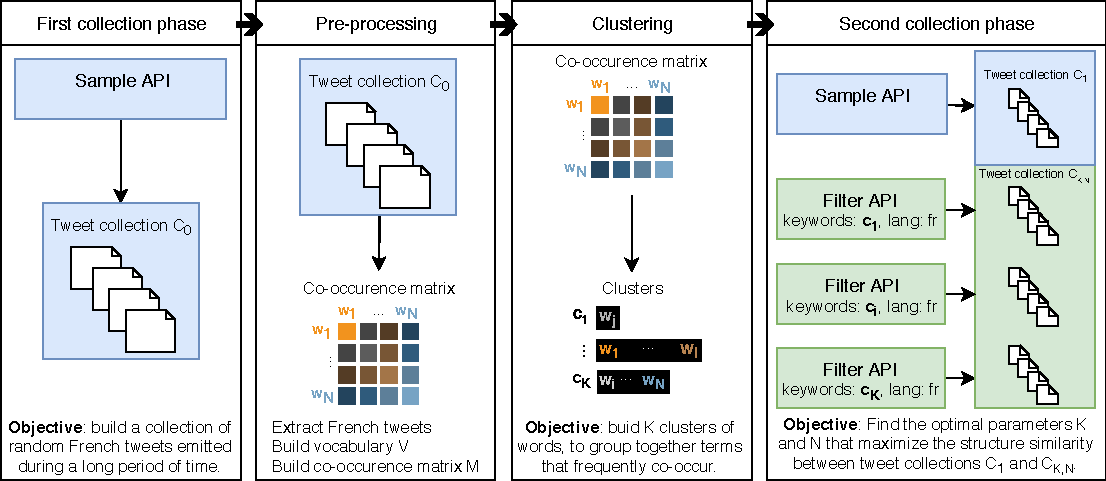
\includegraphics[width=1\textwidth]{figures/Beatrice/ExperimentalSetup.pdf}}
\caption{Diagram of our experimental setup to select the best tweet collection method}
\label{Figure:ExperimentalSetup}
\end{figure}
%%%%%%%%%%%%%%%%%%%%%%%%

%%%%%%%%%%%%%%%%%%%%%%%%
\begin{figure}[h]
\begin{center}
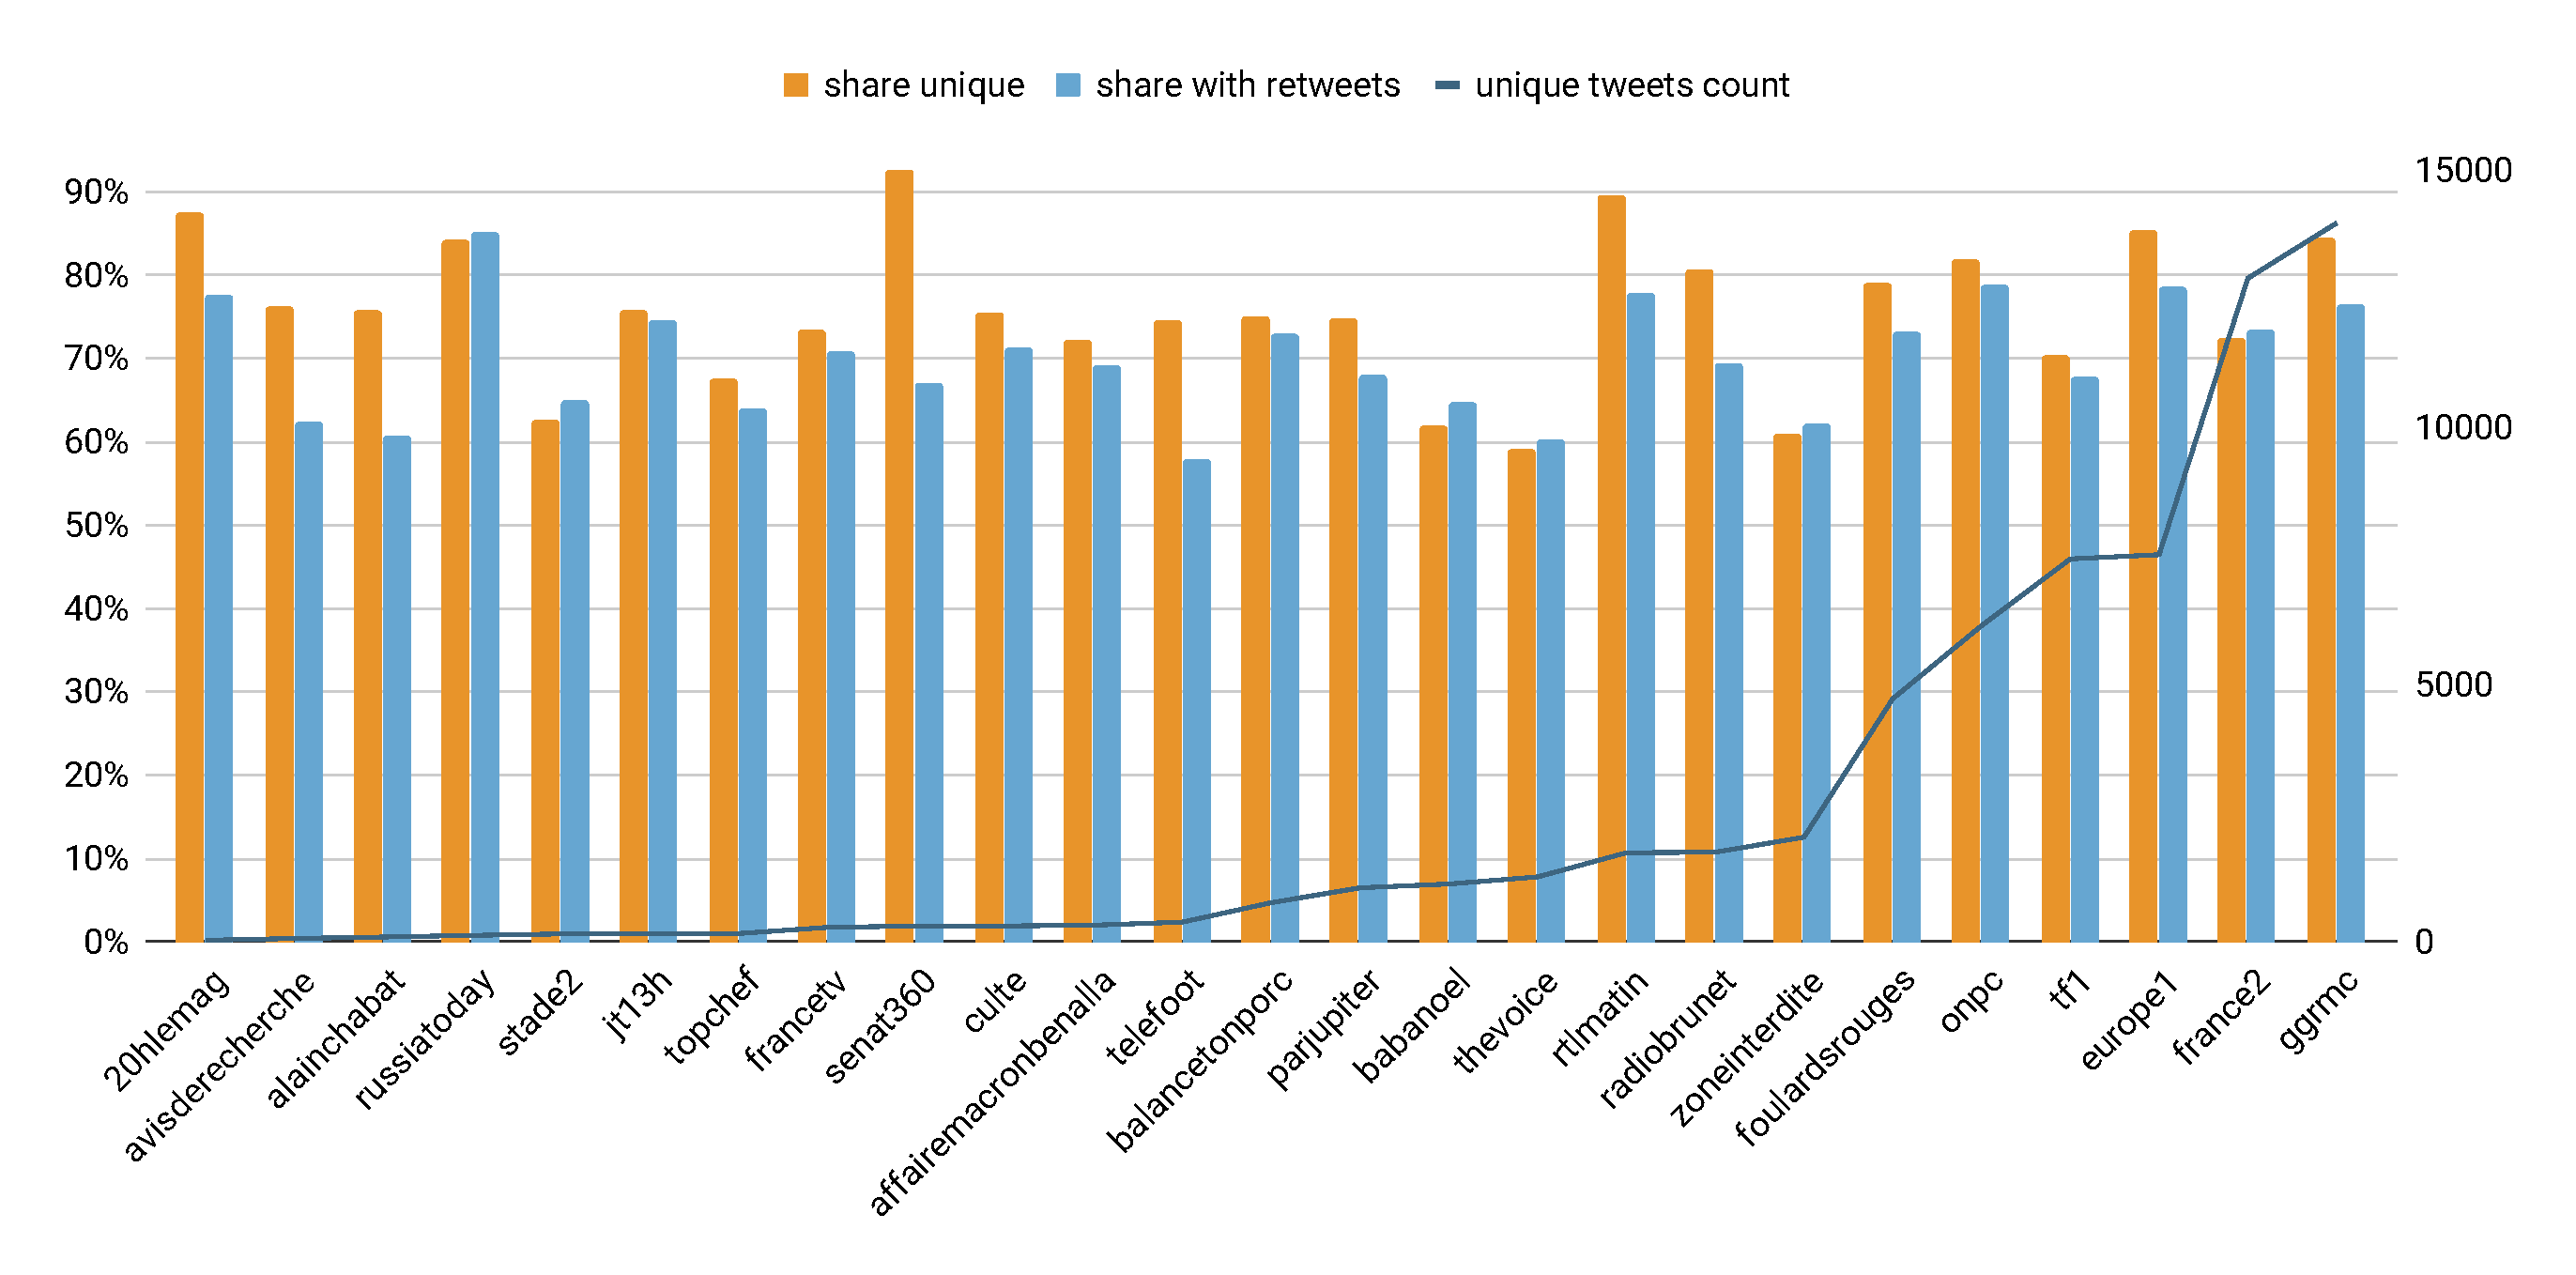
\includegraphics[width=1\textwidth]{figures/Beatrice/ShareinCommonWithDL.pdf}
\end{center}
\scriptsize \textbf{Notes:} This figure plots the share of tweets from the DLWeb that we were also able to capture using our collection method. Blue columns represent the ratio for all tweets, yellow columns represent the ratio for original tweets (\textit{i.e.} retweets excluded). The grey line shows the number of original tweets (\textit{i.e.} retweets excluded) captured by the DLWeb for each hashtag. Tweets were collected from December 1st to December 31st, 2018.
\caption{Share of DLWeb tweets captured using our collection method for a set of 25 hashtags}
\label{Figure:HistogramHashtagsDLWeb}
\end{figure}
%%%%%%%%%%%%%%%%%%%%%%%%


%%%%%%%%%%%%%%%%%%%%%%%%
\begin{figure}[h]
\begin{center}
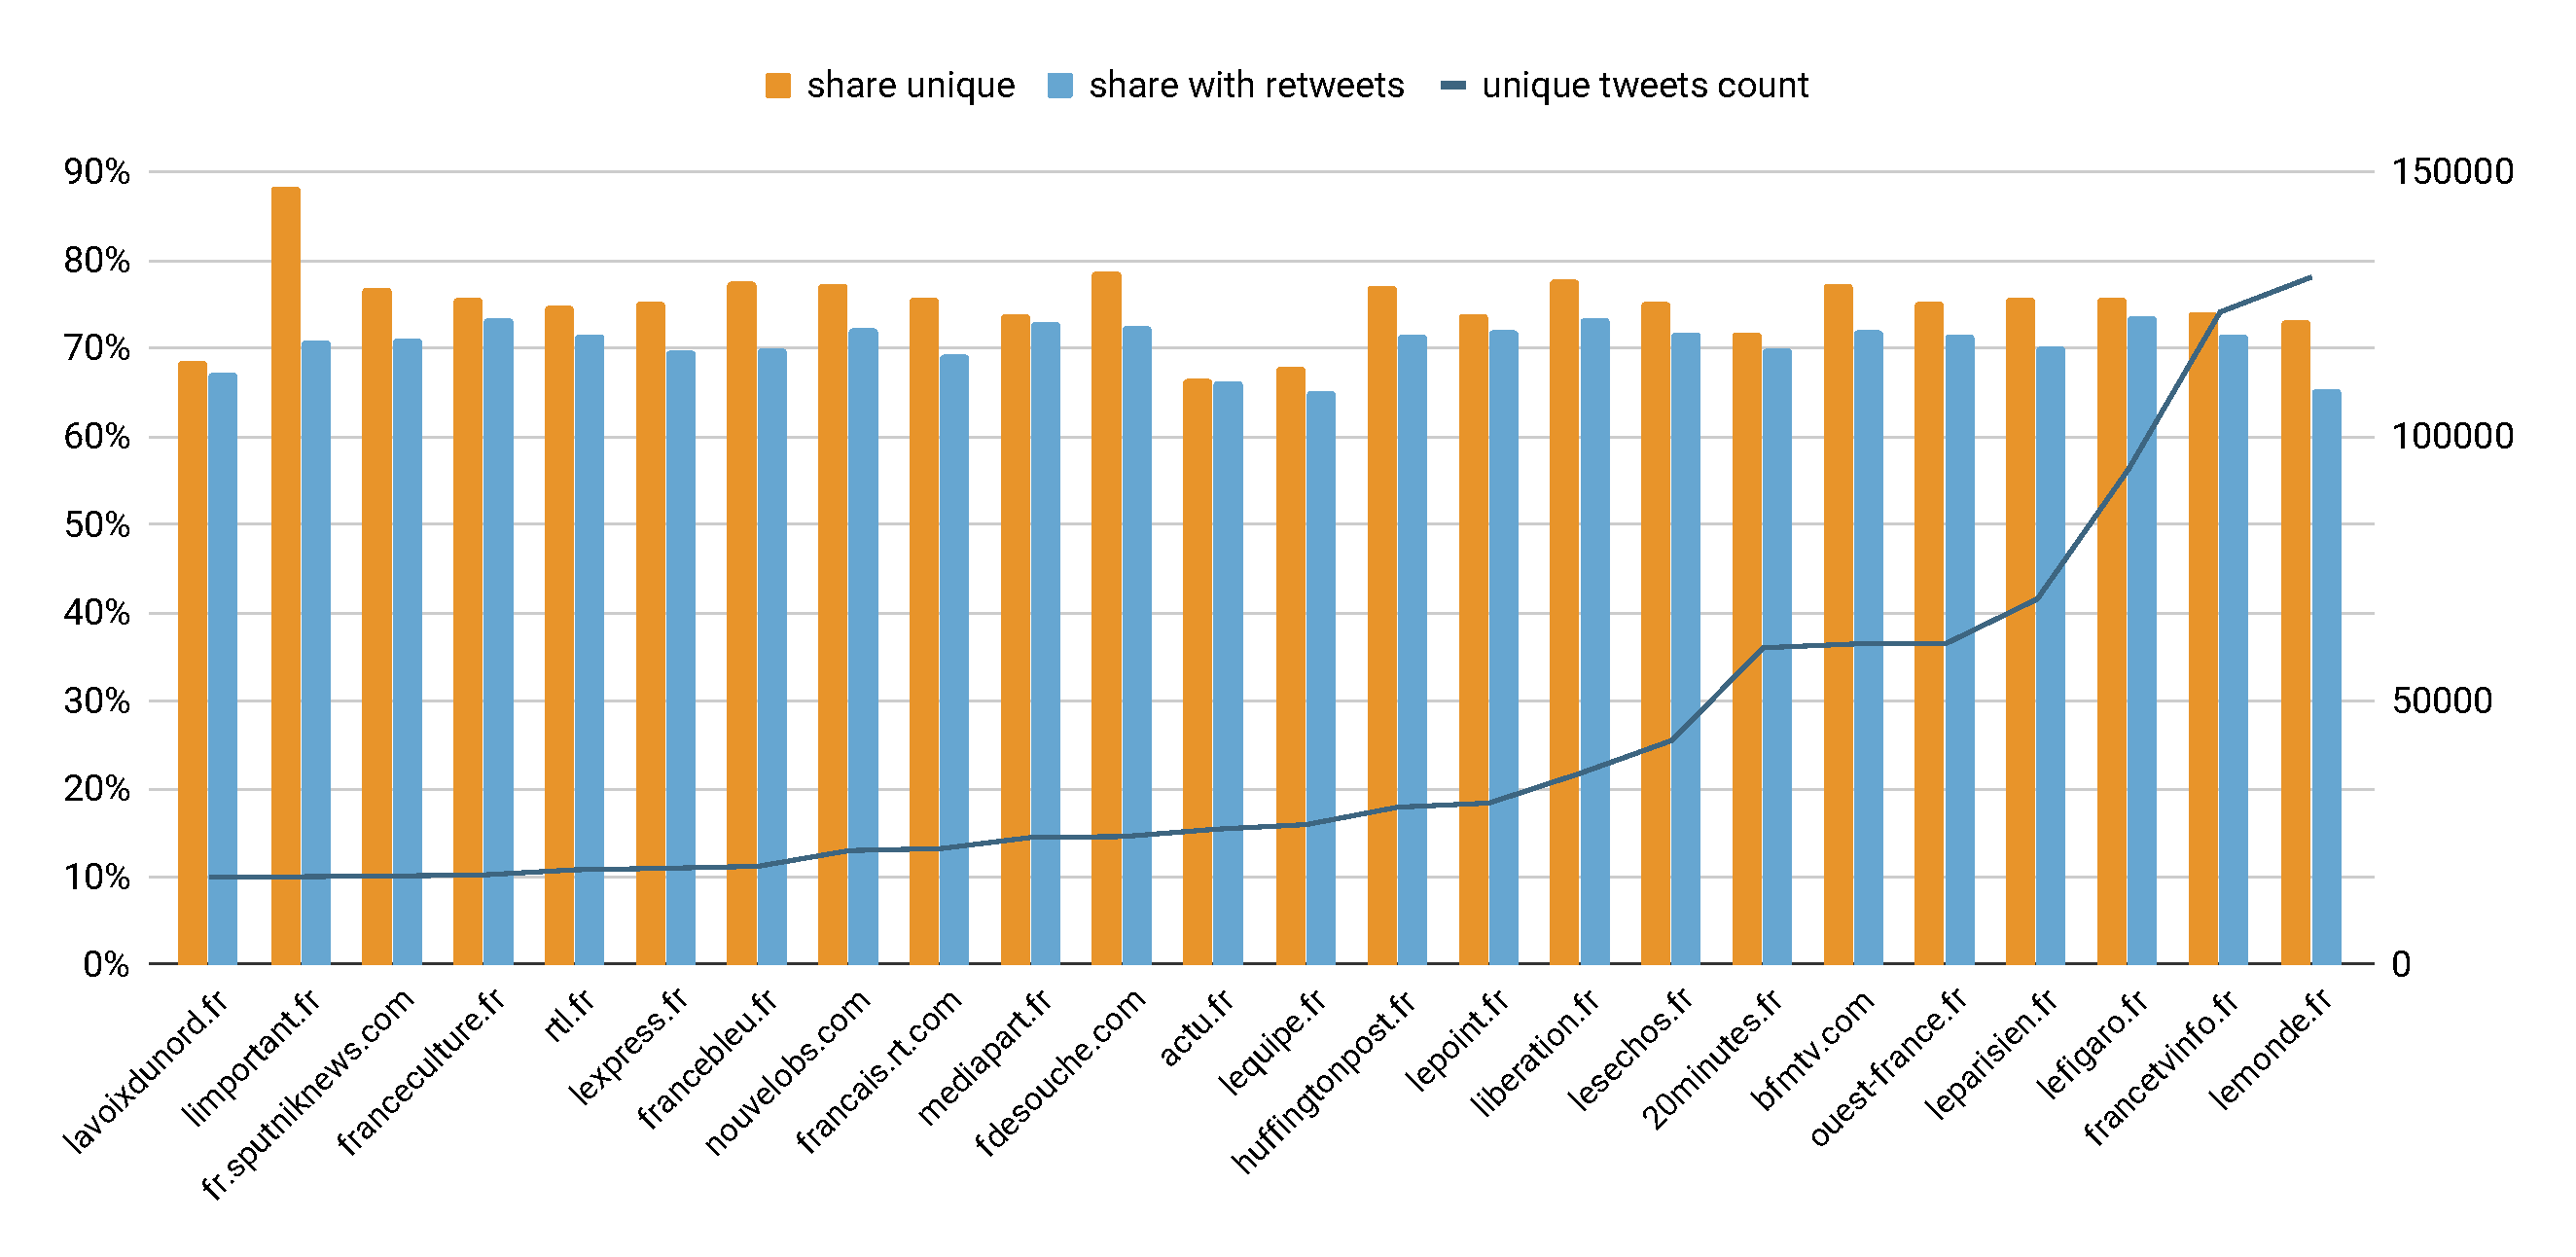
\includegraphics[width=1\textwidth]{figures/Beatrice/ShareInCommonWithMedialab.pdf}
\end{center}
\scriptsize \textbf{Notes:} This figure plots the share of tweets from the Médialab that we were also able to capture using our collection method for the first 25 domain names in terms of original tweets in their dataset. Blue columns represent the ratio for all tweets, yellow columns represent the ratio for original tweets (\textit{i.e.} retweets excluded). The grey line shows the number of original tweets (\textit{i.e.} retweets excluded) captured by the Médialab for each domain. Tweets were collected from December 1st to December 31st, 2018.
\caption{Share of tweets from the Médialab also captured using our collection method for 25 domain names}
\label{Figure:HistogramUrlsMedialab}
\end{figure}
%%%%%%%%%%%%%%%%%%%%%%%%

In order to select users that write mostly in French (tweets written in other languages are not collected with our method), we used the OpenStreetMap API to locate users depending on what they indicate in the ``location" field. We obtained $920,000$ users localized in France that emitted $241$ million tweets in three months, according to the ``number of tweet" field. With our collection method, we captured $147$ million tweets from these users, \textit{i.e.} $61\%$ of the real number of emitted tweets. We found the same percentage with the sample of users who geolocate their tweets in France ($27,000$ users). This method gives us a high estimate of the real number of emitted tweets in French, since some of these users probably write in other languages than French, even if they are located in France.



%%%%%%%%%%%%%%%%%%%%%%%%%%%%%%%%%%%%%%%%%
\paragraph{List of stop words}

To compute the average number of words included in the tweets, we have first removed the stop-words listed in Figure \ref{fig:stop_words}.

%%%%%%%%%%%%%%%%%%%%%%%%%%%%%%%%%%%%%%%%%%%%%%%%%%%%%%%%%%%%%%%%%%%%%%
\begin{figure}[h]
\begin{center}
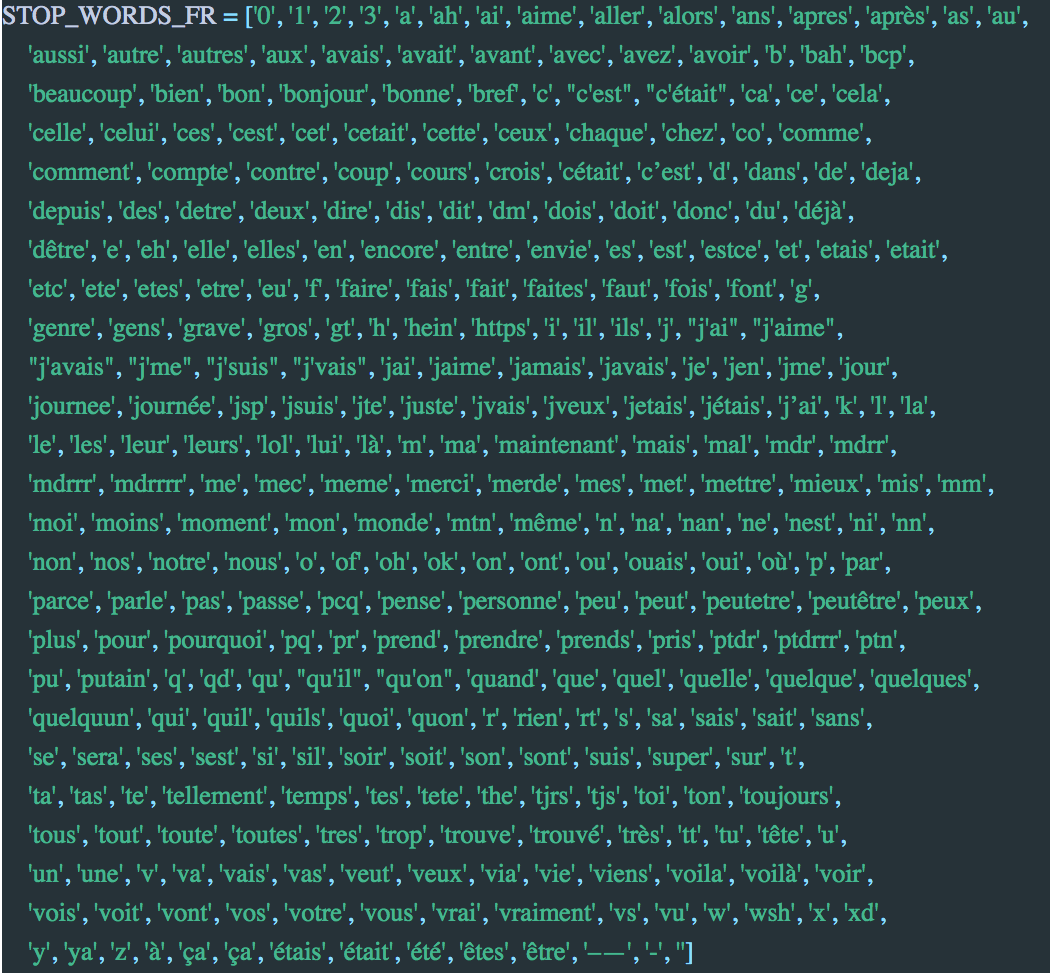
\includegraphics[scale=.7]{figures/stop_words.png}
\end{center}
	\begin{spacing}{0.5}
		{\footnotesize \textbf{Notes:} The figure plots the number of users entering our sample depending on the date of their Twitter account creation.}
	\end{spacing}
\vspace{.5cm}	
	\caption{Twitter users: Number of followers depending on the date of their account creation}
	\label{fig:stop_words}
\end{figure}
%%%%%%%%%%%%%%%%%%%%%%%%%%%%%%%%%%%%%%%%%%%%%%%%%%%%%%%%%%%%%%%%%%%%%% 




%%%%%%%%%%%%%%%%%%%%%%%%%%%%%%%%%%%%%%%%%%
%\paragraph{Identifying accounts of journalists and of media outlets}
%
%To identify the Twitter accounts of journalists and of media outlets, we proceed as follows:
%\textbf{BEATRICE -- A COMPLETER}



%%%%%%%%%%%%%%%%%%%%%%%%%%%%%%%%%%%%%%%%%
\subsection{News media content data\label{Sec:OA_Content}}
%%%%%%%%%%%%%%%%%%%%%%%%%%%%%%%%%%%%%%%%%

The content data is from the OTMedia research projet. This projet was subsidized by the \textit{Agence Nationale de la Recherche} (ANR -- National Agency for Research), a French institution tasked with funding scientific research. The INA (\textit{Institut National de l'Audiovisuel} -- National Audiovisual Institute, a repository of all French radio and television audiovisual archives) was the project leader. The OTMedia research projet used the RSS feeds of the media outlets to track every piece of content they produced online. For the media outlets whose RSS feeds were not tracked by INA, we complete the OTMedia data by scrapping the Sitemaps of their website. Finally, we get all the AFP dispatches (respectively all the Reuters dispatches in French) directly from the AFP (from Reuters).

Our dataset includes the following media outlets:

\begin{multicols}{2}
\textbf{Local daily newspapers:}
	\begin{enumerate}
	\item \textit{L'Ardennais};
	\item  \textit{Aisne Nouvelle};
	\item \textit{Le Berry Republicain};
	\item \textit{La Charente Libre};
	\item \textit{Le Courrier Picard};
	\item \textit{La Depeche Du Midi};
	\item \textit{Est Eclair};
	\item \textit{L'Eveil De La Haute Loire};
	\item \textit{L'Independant Pyrenees Orientales};
	\item \textit{Le Journal De La Haute Marne};
	\item \textit{Le Midi Libre};
	\item \textit{Monaco Matin};
	\item \textit{La Montagne};
	\item \textit{Nice Matin};
	\item \textit{La Nouvelle Republique Des Pyrenees};
	\item \textit{La Nouvelle Republique Du Centre Ouest};
	\item \textit{Ouest France};
	\item \textit{Le Parisien};
	\item \textit{Le Petit Bleu D'Agen};
	\item \textit{La Provence};
	\item \textit{La Republique Des Pyrenees};
	\item \textit{Sud Ouest};
	\item \textit{Le Telegramme};
	\item \textit{L' Union};
	\item \textit{Var Matin};
	\item \textit{La Voix Du Nord};
	\item \textit{Yonne Republicaine}.
	\end{enumerate}
\end{multicols} 	

\begin{multicols}{2}
\textbf{National daily newspapers:}
	\begin{enumerate}
	\item \textit{La Croix};
	\item \textit{Les Echos};
	\item \textit{L'Equipe};
	\item \textit{Le Figaro};
	\item \textit{France Soir};
	\item \textit{La Gazette Des Communes Des Departements Et Des Regions};
	\item \textit{L'Humanite};
	\item \textit{Liberation};
	\item \textit{Le Monde};
	\item \textit{Le Quotidien De L Art};
	\item \textit{La Tribune}.
	\end{enumerate}		
\medskip
\textbf{Free (national daily) newspapers:}
	\begin{enumerate}
	\item \textit{20 Minutes}.
	\end{enumerate}
\medskip
\textbf{Weekly (national \& local) newspapers:}	
	\begin{enumerate}
	\item \textit{10 Sport};
	\item \textit{Agefi};
	\item \textit{Argus};
	\item \textit{Auto Hebdo};
	\item \textit{L'Avenir De Artois};
	\item \textit{Capital};
	\item \textit{Challenges};
	\item \textit{Closer};
	\item \textit{Courrier International};
	\item \textit{Creuse Agricole Et Rurale};
	\item \textit{L'Echo De La Lys};
	\item \textit{Echo Le Valentinois Drome Ardeche};
	\item \textit{Elle};
	\item \textit{Est Agricole Et Viticole};
	\item \textit{L'Express};
	\item \textit{Grazia};
	\item \textit{Les Inrockuptibles};
	\item \textit{Investir};
	\item \textit{Jeune Afrique};
	\item \textit{Le Journal De Millau};
	\item \textit{Le Journal Du Dimanche};
	\item \textit{L'Hebdo Du Vendredi};
	\item \textit{La Manche Libre};
	\item \textit{Marianne};
	\item \textit{Le Monde Diplomatique};
	\item \textit{Le Moniteur Des Travaux Publics Et Du Batiment};
	\item \textit{L'Obs};
	\item \textit{L'Observateur De Beauvais};
	\item \textit{Paris Match};
	\item \textit{Le Paysan Du Haut Rhin};
	\item \textit{Le Point};
	\item \textit{Point De Vue};
	\item \textit{Le Republicain De L'Essonne};
	\item \textit{La Semaine Dans Le Boulonnais};
	\item \textit{Strategies};
	\item \textit{Tele Z};
	\item \textit{L'Usine Nouvelle};
	\item \textit{Version Femina};
	\item \textit{La Volonte Paysanne De L'Aveyron}.
	\end{enumerate}
\medskip	
\textbf{Monthly (national) newspapers:}
	\begin{enumerate}
	\item \textit{Auto Infos};
	\item \textit{Beaux Arts};
	\item \textit{Causeur};
	\item \textit{Connaissance Des Arts};
	\item \textit{Le Courrier De Floride Etats Unis};
	\item \textit{France Amerique Etats Unis};
	\item \textit{Geo};
	\item \textit{GQ Magazine};
	\item \textit{Japon Infos};
	\item \textit{Marie Claire};
	\item \textit{Marie France};
	\item \textit{Mon Viti};
	\item \textit{Premiere};
	\item \textit{Rav};
	\item \textit{La Revue Des Deux Mondes};
	\item \textit{Science Et Vie};
	\item \textit{Sciences Et Avenir};
	\item \textit{Sciences Humaines};
	\item \textit{Tarx};
	\item \textit{Tetu};
	\item \textit{Vogue};
	\item \textit{Zibeline}.
	\end{enumerate}		
\medskip
\textbf{TV:}
	\begin{enumerate}
	\item BFM TV;
	\item Eurosport;
	\item France 24;
	\item LCI;
	\item Public Senat;
	\item TF1;
	\item TV5 Monde.
	\end{enumerate}
\medskip
\textbf{Radio:}
	\begin{enumerate}
	\item Europe 1;
	\item France Bleu (Radio France);
	\item France Culture (Radio France);
	\item France Inter (Radio France);
	\item France Musique (Radio France);
	\item France Info (also TV);
	\item Radio Classique;
	\item RCF;
	\item RFI;
	\item RTL;
	\item Tendance Ouest.
	\end{enumerate}				
\medskip
\textbf{News agencies:} 
	\begin{enumerate}
	\item Agence France Presse.
%	\item Reuters. \textbf{A RAJOUTER}
	\end{enumerate}	
\medskip
\textbf{Pure online media:}
	\begin{enumerate}
	\item 01 Net;
	\item Actu;
	\item Aleteia;
	\item AOC;
	\item Arboriculture Fruitiere;
	\item Basta;
	\item Boursier Com;
	\item Boursorama;
	\item Bref Eco;
	\item Buzzfeed;
	\item C Net;
	\item Cfnews;
	\item Clubic;
	\item Contrepoints;
	\item Les Echos Du Touquet;
	\item Echos Start;
	\item Echosdunet;
	\item Foot Mercato;
	\item Football;
	\item Gamekult;
	\item Gamergen;
	\item Generation Nouvelles Technologies;
	\item Ginjfo;
	\item Goodplanet Info;
	\item Herault Tribune;
	\item Huffington Post;
	\item Influenth;
	\item Informatique News;
	\item L'ADN;
	\item Le Libre Penseur;
	\item Le Media;
	\item Le Tribunal Du Net;
	\item L'Explicite;
	\item L'Incorrect;
	\item L'Internaute;
	\item LVSL;
	\item Maddyness;
	\item Made In Foot;
	\item Made In Perpignan;
	\item Marsactu;
	\item Mashable;
	\item Medialot;
	\item Mediapart;
	\item Meta Media;
	\item Minutenews;
	\item Mon Cultivar Elevage;
	\item Mondafrique;
	\item Monde Informatique;
	\item Les Moutons Enrages;
	\item Myeurop Info;
	\item Newsly;
	\item Numerama;
	\item Numeriques;
	\item Ohmymag;
	\item Olivieranger;
	\item Paris Depeches;
	\item Le Petit Journal;
	\item Pourquoi Docteur;
	\item Pure Medias;
	\item Purepeople;
	\item Resistance Republicaine;
	\item Rue 89 Lyon;
	\item Rue89 Bordeaux;
	\item Rue89 Strasbourg;
	\item Slate;
	\item Sputniknews;
	\item Toulouse 7;
	\item Toute La Culture;
	\item La Tribune De L Art;
	\item Up Magazine;
	\item L'Usine Digitale.
	\end{enumerate}			
\end{multicols}


%%%%%%%%%%%%%%%%%%%%%%%%%%%%%%%%%%%%%%%%%
\paragraph{French-speaking foreign media}

Further, we also gather the content produced online by the following French-speaking foreign media:
\begin{enumerate}
\item \textit{20 Minutes Suisse} (Switzerland);
\item Quotidien Canada (Canada);
\item \textit{Temps Suisse} (Switzerland);
\item Lequotidien (pure online media from Quebec);
\item Africa Intelligence;
\item Express Mu Ile Maurice;
\item Nouvelles Caledoniennes;
\item Nouvelle Tribune Benin;
\item Wort Luxembourg;
\item Infohaiti Net Haiti.
\end{enumerate}


%%%%%%%%%%%%%%%%%%%%%%%%%%%%%%%%%%%%%%%%%
\subsection{IPTC topics\label{Sec:OATopic}}
%%%%%%%%%%%%%%%%%%%%%%%%%%%%%%%%%%%%%%%%%

To define the subject of its dispatches, AFP uses URI, available as QCodes, designing 17 IPTC media topics. The IPTC is the International Press Telecommunications Council. 

The 17 topics are defined as follows:

\begin{itemize}
\item \textbf{Arts, culture and entertainment}: matters pertaining to the advancement and refinement of the human mind, of interests, skills, tastes and emotions.
\item \textbf{Crime, law and justice}: establishment and/or statement of the rules of behaviour in society, the  enforcement of these rules, breaches of the rules and the punishment of offenders.
Organisations and bodies involved in these activities. 
\item \textbf{Disaster and accident}: man made and natural events resulting in loss of life or injury to living creatures and/or damage to inanimate objects or property.
\item \textbf{Economy, business and finance}: all matters concerning the planning, production and exchange of wealth.  
\item \textbf{Education}: all aspects of furthering knowledge of human individuals from birth to death.
\item \textbf{Environment}: all aspects of protection, damage, and condition of the ecosystem of the planet earth and its surroundings.
\item \textbf{Health}: all aspects pertaining to the physical and mental welfare of human beings. 
\item \textbf{Human interest}: items about individuals, groups, animals, plants or other objects with a focus on emotional facets.
\item \textbf{Labour}: social aspects, organisations, rules and conditions affecting the employment of human effort for the generation of wealth or provision of services and the economic support of the unemployed.
\item \textbf{Lifestyle and leisure}: activities undertaken for pleasure, relaxation or recreation outside paid employment, including eating and travel.
\item \textbf{Politics}: local, regional, national and international exercise of power, or struggle for power, and the relationships between governing bodies and states.
\item \textbf{Religion and belief}: all aspects of human existence involving theology, philosophy, ethics and spirituality.
\item \textbf{Science and technology}: all aspects pertaining to human understanding of nature and the physical world and the development and application of this knowledge.
\item \textbf{Society}: aspects of the life of humans affecting its relationships.
\item \textbf{Sport}: competitive exercise involving physical effort. Organizations and bodies involved in these activities.
\item \textbf{Conflicts, war and peace}: acts of socially or politically motivated protest and/or violence and actions to end them. 
\item \textbf{Weather}: the study, reporting and prediction of meteorological phenomena.
\end{itemize}                               



\clearpage 
%%%%%%%%%%%%%%%%%%%%%%%%%%%%%%%%%%%%%%%%%
%%%%%%%%%%%%%%%%%%%%%%%%%%%%%%%%%%%%%%%%%
\section{Algorithms\label{Sec:Algorithms}}
%%%%%%%%%%%%%%%%%%%%%%%%%%%%%%%%%%%%%%%%%
%%%%%%%%%%%%%%%%%%%%%%%%%%%%%%%%%%%%%%%%%


%%%%%%%%%%%%%%%%%%%%%%%%%%%%%%%%%%%%%%%%%
\subsection{Social media event detection\label{Sec:SME_algo}}
%%%%%%%%%%%%%%%%%%%%%%%%%%%%%%%%%%%%%%%%%

%%%%%%%%%%%%%%%%%%%%%%%%%%%%%%%%%%%%%%%%%%%%%%
\paragraph{Preprocessing}
  
Each text embedding model takes different text formats as inputs: for example, models able to deal with sentences, such as BERT, Sentence-BERT, ELMo or Universal Sentence Encoder, take the full text with punctuation as input. For Word2Vec and tf-idf models, we lowercase characters and remove punctuation. Table \ref{Tab:preprocessing} summarizes all preprocessing steps depending on the type of model. Each column corresponds to a preprocessing step:

\begin{itemize}
\item Remove mentions: mentions are a Twitter-specific way of referring to another Twitter user in a tweet, so that she is notified that the tweet is talking about her or is addressed to her. Entries take the following form: @name\_of\_the\_user. For tf-idf models, removing mentions is a way to reduce the size of the vocabulary. For most Word2Vec models, mentions are not part of the vocabulary, except for w2v\_twitter\_en.
\item Unidecode: we use the Python module unidecode to convert Unicode characters to ASCII characters. In French, for example, all accents are removed: ``Wikip\'{e}dia" becomes ``Wikipedia".
\item Lower: we set the text in lowercase letters.
\item Hashtag split: we split hashtags on capital letters. ``\#HappyEaster" becomes "Happy Easter". This step is of course applied before lowercasing.
\item Remove long numbers: we remove numbers longer than 4 digits.
\item Remove repeated characters: we limit the number of repeated characters inside a word to three. ``looooool" becomes ``loool".
\end{itemize}

%%%%%%%%%%%%%%%%%%%%%%%%%%%%
\begin{sidewaystable}
\begin{center}
\makebox[\textwidth][c]{\begin{tabular}{lcccccccc}
\hline
                 model & rm mentions & unidecode & lower & rm punctuation & hashtag split & rm long numbers & rm repeated chars & rm urls \\
\hline
      tfidf\_all\_tweets &           X &         X &     X &              X &             X &               X &                 X &       X \\
         tfidf\_dataset &           X &         X &     X &              X &             X &               X &                 X &       X \\
            w2v\_afp\_fr &           X &         X &     X &              X &             X &               X &                 X &       X \\
        w2v\_twitter\_fr &           X &         X &     X &              X &             X &               X &                 X &       X \\
          w2v\_gnews\_en &           X &           &       &              X &             X &               X &                 X &       X \\
        w2v\_twitter\_en &             &           &       &              X &             X &               X &                 X &       X \\
                  elmo &             &           &       &                &             X &               X &                 X &       X \\
                  bert &             &           &       &                &             X &               X &                 X &       X \\
           bert\_tweets &             &           &       &                &             X &               X &                 X &       X \\
             sbert\_sts &             &           &       &                &             X &               X &                 X &       X \\
         sbert\_nli\_sts &             &           &       &                &             X &               X &                 X &       X \\
      sbert\_tweets\_sts &             &           &       &                &             X &               X &                 X &       X \\
 sbert\_tweets\_sts\_long &             &           &       &                &             X &               X &                 X &       X \\
                   use &             &           &       &                &             X &               X &                 X &       X \\
\hline
\end{tabular}
}
\end{center}
\caption{Preprocessing applied for each model \label{Tab:preprocessing}}
\end{sidewaystable}
%%%%%%%%%%%%%%%%%%%%%%%%%%%%



%%%%%%%%%%%%%%%%%%%%%%%%%%%%%%%%%%%%%%%%%
\subsection{Mainstream media event detection algorithm\label{Sec:event_algo}}
%%%%%%%%%%%%%%%%%%%%%%%%%%%%%%%%%%%%%%%%%

%%%%%%%%%%%%%%%%%%%%%%%%%%%%%%%%%%%%%%%%%%%%%%
\paragraph{Description of the algorithm}

The goal of online topic detection is to organize a constantly arriving stream of news articles by the events they discuss. The algorithms place all the documents into appropriate and coherent clusters. Consistency is ensured both at the temporal and the semantic levels. As a result, each cluster provided by the algorithm covers the same topic (event) and only that topic. Following \citet{Allan2005} who have experienced their TDT system in a real world situation, we adopt the following implementation:

\begin{enumerate}
\item As in most natural language processing methods, we first pre-process our documents by removing very common words (called stop words) and applying a stemming algorithm so as to keep only the stem of the words.

\item Each document is then described by a semantic vector which takes into account both the headline and the text. We apply a multiplicative factor of five to the words of the title as they are supposed to describe the event well, resulting in an overweight in the global vector describing the document. A semantic vector represents the relative importance of each word of the document compared to the full dataset. A standard scheme is TF-IDF: term frequency-inverse document frequency, a numerical statistic intended to reflect how important a word is to a document in a corpus. The TF-IDF value increases proportionally to the number of times a word appears in the document, but is offset by the frequency of the word in the corpus. More precisely, the weight of a word $w$ in a document $d$ is: $TFIDF(w,d) = wf\left(w,d\right)*log\left(N/df\left(w\right)\right)$, where $wf$ is the frequency of word $w$ in the considered document, $dw$ is the number of documents in which it appears, and $N$ is the total number of documents. The total vector is $TFIDF(d) = \left[TFIDF(w_{1},d),TFIDF(w_{2},d),..., TFIDF(w_{n},d)\right]$, where $w_{1},..., w_{n}$ are the words occurring in the whole text stream to segment.

\item The documents are then clustered in a bottom-up fashion to form the events based on their semantic similarity. The similarity between two documents is given by the distance between their two semantic vectors. We use the cosine similarity measure \citep{Salton1975}.

\item This iterative agglomerative clustering algorithm is stopped when the distance between documents reaches a given threshold. We have determined this threshold empirically based on manually created media events.

\item A cluster is finalized if it does not receive any new document for a given period of time. We use a one-day window.\footnote{Events can last more than one day. But if during a 24-hour period of time no document is placed within the cluster, then the cluster is closed. Any new document published after this time interval becomes the seed of a new event cluster.} 
\end{enumerate}


%%%%%%%%%%%%%%%%%%%%%%%%%%%%%%%%%%%%%%%%%%%%%%
\paragraph{Performance of the algorithm}

This event detection algorithm can be compared to other detection systems by its ability to put all the stories in a single event together. We test the quality of the algorithm by running it on a standard benchmark dataset: the Topic Detection and Tracking (TDT) Pilot Study Corpus. The TDT dataset contains events that have been created ``manually": the goal is to compare the performance of the algorithm with that of humans. The goal of the TDT initiative is to investigate the state of the art in finding and following events in a stream of news stories \citep[see e.g.][]{Allan1998}. To test the performance of our algorithm on the English corpus, we slightly adapt it. There is indeed no similar test corpus in French. First, we use an English stop-word list and an English stemming algorithm. Second, the time frame of the test corpus being wider than ours, the one-day window used to close clusters is not adapted. When testing our algorithm we thus follow the literature \citep{Allan2005} and close a cluster when $2,500$ documents have been treated by the algorithm and none of them has been added to the cluster.

In the TDT Pilot Study \citet{Allan1998}, two types of algorithms are evaluated: a ``retrospective algorithm" and an ``online algorithm". A retrospective algorithm needs to know all the articles in order to detect media events whereas an online algorithm is fed by the stream of articles, one by one. Given that the OTMedia platform must be able to manage articles in real time, we implemented an online algorithm. 

%Two measures are used in the official evaluation to estimate the performance of the algorithms: micro and macro average F1. These are standard measures in the information retrieval field that combine precision and recall. We report in Figure \ref{fig:fig_run} the best runs from \citet{Allan1998}. The performances of our algorithm clearly outperform the best online algorithm of \citet{Allan1998}. Moreover, despite being online, and thus having less information available, our results are only $10\%$ behind the retrospective implementation.
%
%
%%%%%%%%%%%%%%%%%%%%%%%%%%%%%%%%%%%%%%%%%%%%%%%%%%%%%%%%%%%%%%%%%%%%%%%%
%\begin{figure}
%\begin{center}
%\includegraphics[scale=1]{../../../../../../../../figures/fig_run.pdf}
%\end{center}
%\begin{spacing}{0.5}
%{\fns \textbf{Notes:} The figure reports the micro and macro average F1 statistics of three algorithms: the best retrospective (Retrospective CMU incremental) and online (Online CMU decay -- win2500) algorithms of \citet{Allan1998}, and our online algorithm. CMU stands for Carnegie Mellon University, where the best algorithms of \citet{Allan1998} have been implemented.}
%\end{spacing}
%\vspace{.5cm}
%\caption{performance of the algorithms: micro and macro average F1}
%\label{fig:fig_run}
%\end{figure}
%%%%%%%%%%%%%%%%%%%%%%%%%%%%%%%%%%%%%%%%%%%%%%%%%%%%%%%%%%%%%%%%%%%%%%%%


Note also that we find that the main parameter of our implementation, the distance threshold on semantic similarity, is the same for this English test corpus and our corpus of French news articles. While we were expecting these thresholds to be of similar order of magnitude (the TF-IDF representation of text is only based on word appearance frequencies; given both corpuses include articles that are of the same nature, it is not surprising to obtain relatively close thresholds for French and English), finding a similar threshold is nonetheless very reassuring as to the quality of our algorithm. In particular, it ensures that the news events that are detected by our algorithm are as close as possible to what a human would be able to do.



%%%%%%%%%%%%%%%%%%%%%%%%%%%%%%%%%%%%%%%%%
%\subsection{Plagiarism detection algorithm\label{Sec:event_plagia}}
%%%%%%%%%%%%%%%%%%%%%%%%%%%%%%%%%%%%%%%%%
%
%A RAJOUTER QUAND ON AURA LES DONNEES
%
%The plagiarism detection algorithm tracks efficiently identical portions of text between documents. Technically, the algorithm is based on \textit{hashing} techniques of n-grams (the n-grams consist in sets of n consecutive words, we use 5-grams) and a threshold on the minimal length of a shared text portion to consider there is a copy (we use 100 characters). We use an \textit{hashing}-based technique to save processing times \citep[see e.g.][]{Stein2007}. \textit{Hashing} is a technique used for rapid calculation of distances in vector spaces. This technique addresses the completeness of the search to save processing time. The space is divided into portions, and the research is conducted on a subset of these portions.
%
%We focus on exact (verbatim) copying only. For each document, we determine the portions of text that are identical to content previously published by all the documents out earlier in the event, and isolate the original content in the document. The originality rate of a document is defined as the share of the document's content (in number of characters) that is original.
%
%Moreover, we trace back each portion of text to its first occurrence in the event. It allows us to determine for each document the number of times it is copied and the share of the document which is ultimately copied. 



%%%%%%%%%%%%%%%%%%%%%%%%%%%%%%%%%%%%%%%%%
\subsection{Joint events\label{Sec:Joint_events}}
%%%%%%%%%%%%%%%%%%%%%%%%%%%%%%%%%%%%%%%%%

\textbf{BEATRICE} -- decrire en details la methode utilisee pour les evenements joints


%%%%%%%%%%%%%%%%%%%%%%%%%%%%%%%%%%%%%%%%%%%%%%%%%%%%%%%%%%%%%%%%%%%%%%
\begin{figure}
\begin{center}
	\subfloat[][\textbf{ Building the similarity network}]{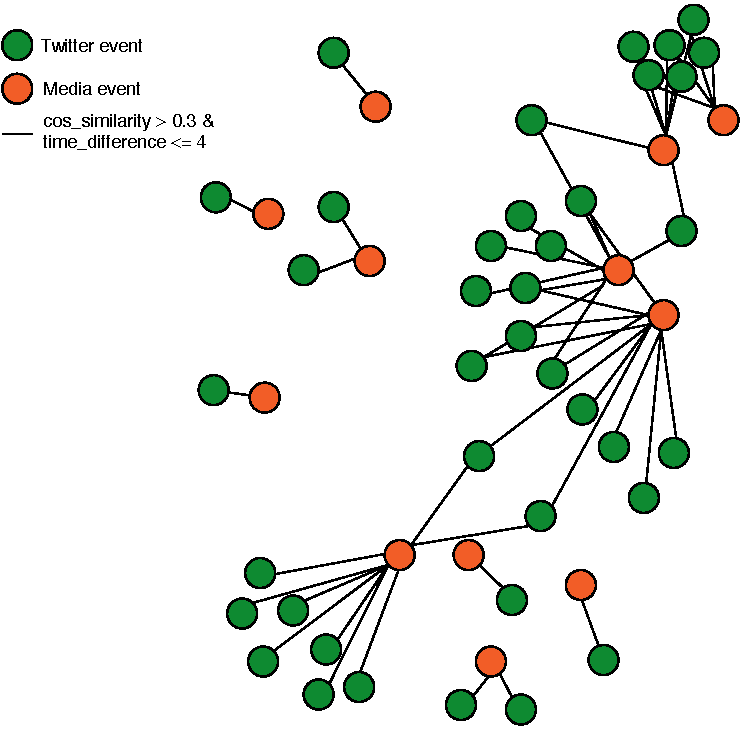
\includegraphics[scale=.7]{figures/GraphMediaEvents}
\label{fig:GraphMediaEvents}}
\quad
	\subfloat[][\textbf{Applying Louvain algorithm}]{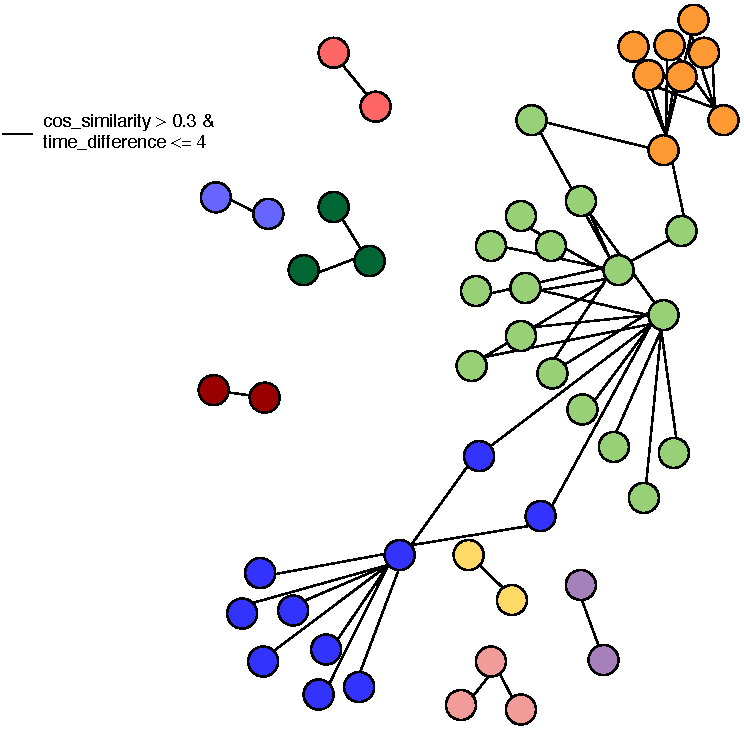
\includegraphics[scale=.7]{figures/GraphCommunityDetection}
\label{fig:GraphCommunityDetection}}
\end{center}
	\begin{spacing}{0.5}
		{\footnotesize \textbf{Notes:} \textbf{A COMPLETER}.}
	\end{spacing}
\vspace{.5cm}	
	\caption{Graphical representation: Building the joint events}
	\label{fig:users}
\end{figure}
%%%%%%%%%%%%%%%%%%%%%%%%%%%%%%%%%%%%%%%%%%%%%%%%%%%%%%%%%%%%%%%%%%%%%% 



\clearpage 
\pagebreak
%%%%%%%%%%%%%%%%%%%%%%%%%%%%%%%%%%%%%%%%%
%%%%%%%%%%%%%%%%%%%%%%%%%%%%%%%%%%%%%%%%%
\section{Additional tables \label{Sec:AdTables}}
%%%%%%%%%%%%%%%%%%%%%%%%%%%%%%%%%%%%%%%%%
%%%%%%%%%%%%%%%%%%%%%%%%%%%%%%%%%%%%%%%%%

%%%%%%%%%%%%%%%%%%%%%%%%%%%%%%%%%%%%%%%%%%%%%%%%%%%%%%%%%%%%%%%%%%%%%%
\begin{sidewaystable}
\caption{Summary statistics: Tweets -- split sample (July 2018 - September 2018), before filters}
\begin{center}
	{
\def\sym#1{\ifmmode^{#1}\else\(^{#1}\)\fi}
\begin{tabular}{l*{1}{ccccccc}}
\hline\hline
                    &\multicolumn{7}{c}{}                                                                      \\
                    &        Mean&      St.Dev&         P25&      Median&         P75&         Max&         Obs\\
\hline
\textbf{Characteristics of the tweet}&            &            &            &            &            &            &            \\
Length of the tweet (nb of characters)&         101&          52&          60&          97&         140&       1,121& 428,338,133\\
Number of words     &         6.2&         4.0&         3.0&         6.0&         8.0&         269& 428,338,133\\
=1 if tweet contains an URL&        0.13&        0.33&       0.000&       0.000&       0.000&           1& 428,338,133\\
=1 if the tweet is a retweet&        0.63&        0.48&       0.000&       1.000&       1.000&           1& 428,338,133\\
=1 if the tweet is a reply&        0.17&        0.38&       0.000&       0.000&       0.000&           1& 428,338,133\\
=1 if the tweet is a quote&        0.19&        0.39&       0.000&       0.000&       0.000&           1& 428,338,133\\
\textbf{Popularity of the tweet}&            &            &            &            &            &            &            \\
Number of retweets  &         2.2&       110.4&       0.000&       0.000&       0.000&     117,389& 159,932,748\\
Number of replies   &         0.2&         6.5&       0.000&       0.000&       0.000&      47,892& 159,932,748\\
Number of likes     &         3.7&       177.6&       0.000&       0.000&       0.000&     449,881& 159,932,749\\
\hline\hline
\end{tabular}
}

\end{center}
\begin{spacing}{0.5}
	{\fns \textbf{Notes:} The table gives summary statistics. Time period is July 2018 - September 2018. Variables are values for all the tweets included in our dataset before we applied the filters to remove the bots. Variables are described in more details in the text.} 
\end{spacing}
\label{Tab:sum_stat_tweets_split_sample_bflitre}
\end{sidewaystable} 
%%%%%%%%%%%%%%%%%%%%%%%%%%%%%%%%%%%%%%%%%%%%%%%%%%%%%%%%%%%%%%%%%%%%%%


%%%%%%%%%%%%%%%%%%%%%%%%%%%%%%%%%%%%%%%%%%%%%%%%%%%%%%%%%%%%%%%%%%%%%%
\begin{sidewaystable}[h]
\caption{Summary statistics: Twitter users (full sample; last time the user is observed)}
\begin{center}
	{
\def\sym#1{\ifmmode^{#1}\else\(^{#1}\)\fi}
\begin{tabular}{l*{1}{cccccc}}
\hline\hline
                    &\multicolumn{6}{c}{}                                                         \\
                    &        Mean&      St.Dev&         P25&      Median&         P75&         Max\\
\hline
\textbf{User activity}&            &            &            &            &            &            \\
Total number of tweets&      15,174&      40,642&         286&       2,265&      12,762&   6,183,567\\
Nb of tweets btw first \& last time&          99&         445&           4&           9&          38&      61,203\\
Nb of tweets user has liked&       8,520&      23,184&         158&       1,220&       6,655&   2,831,010\\
Nb of users the account is following&         688&        4549&          88&         211&         519&     1672425\\
\textbf{User identity}&            &            &            &            &            &            \\
Date of creation of the account&   2,014.469&       2.742&       2,012&       2,015&       2,017&       2,018\\
=1 if verified account&       0.005&       0.074&           0&           0&           0&           1\\
=1 if user is a journalist&      0.0012&       0.034&           0&           0&           0&           1\\
=1 if user is a media&           0&           0&           0&           0&           0&           1\\
\textbf{User popularity}&            &            &            &            &            &            \\
Nb of followers     &       2,200&      86,685&          32&         147&         515&  58,775,462\\
Nb of public lists  &          20&         578&           0&           1&           6&   1,028,438\\
\hline
Observations        &   4,222,734&            &            &            &            &            \\
\hline\hline
\end{tabular}
}

\end{center}
\begin{spacing}{0.5}
	{\fns \textbf{Notes:} The table gives summary statistics. Time period is July 2018 - July 2019. Variables are values for all the Twitter users included in our dataset the last time we observe them. Variables are described in more details in the text.} 
\end{spacing}
\label{Tab:table_summary_users_all_last}
\end{sidewaystable} 
%%%%%%%%%%%%%%%%%%%%%%%%%%%%%%%%%%%%%%%%%%%%%%%%%%%%%%%%%%%%%%%%%%%%%%


%%%%%%%%%%%%%%%%%%%%%%%%%%%%
%\clearpage 
%\pagebreak
%\begin{table}
%\caption{Summary statistics: Tweets in SMEs and not in SMEs}
%\begin{center}
%{
\def\sym#1{\ifmmode^{#1}\else\(^{#1}\)\fi}
\begin{tabular}{l*{1}{ccc}}
\hline\hline
                    &\multicolumn{3}{c}{ }                          \\
                    &Not in event&    In event&     Diff/se         \\
\hline
\textbf{Characteristics of the tweet}&            &            &                     \\
Length of the tweet (nb of characters)&         134&          73&          61\sym{***}\\
                    &            &            &       (0.0)         \\
Number of words     &           9&           5&           4\sym{***}\\
                    &            &            &       (0.0)         \\
=1 if tweet contains an URL&         0.1&         0.2&      -0.037\sym{***}\\
                    &            &            &     (0.000)         \\
\textbf{Popularity of the tweet}&            &            &                     \\
Number of retweets  &         1.8&         2.5&        -0.7\sym{***}\\
                    &            &            &       (0.0)         \\
Number of replies   &         0.2&         0.2&        -0.0\sym{***}\\
                    &            &            &       (0.0)         \\
Number of likes     &         3.0&         3.8&        -0.8\sym{***}\\
                    &            &            &       (0.0)         \\
\hline
Observations        & 114,698,415&            &                     \\
\hline\hline
\end{tabular}
}

%\end{center} 
%	\begin{spacing}{0.5}
%	{\scriptsize \textbf{Notes:} * p$<$0.10, ** p$<$0.05, *** p$<$0.01. The tables give summary statistics 
%for the characteristics of the tweets in our sample. Time period is July 2018 - September 2018. Column 1 presents the results for the tweets not included in social media events. Column 2 presents the results for the tweets included in social media events. In column 3, we perform a \textit{t}-test on the equality of means.}
%	\end{spacing}
%\label{Tab:sum_stat_tweets_ttest}
%\end{table}
%%%%%%%%%%%%%%%%%%%%%%%%%%%%


%%%%%%%%%%%%%%%%%%%%%%%%%%%%%%%%%%%%%%%%%%%%%%%%%%%%%%%%%%%%%%%%%%%%%%
\begin{table}
\caption{Summary statistics: Joint events -- Depending on news breaker\label{Tab:table_summary_joint_events_ttest}}
\begin{center}
{
\def\sym#1{\ifmmode^{#1}\else\(^{#1}\)\fi}
\begin{tabular}{l*{1}{ccc}}
\hline\hline
                    &\multicolumn{3}{c}{ }                          \\
                    & Media first&Twitter first&     Diff/se         \\
\hline
Length of the event (in hours)&         408&         529&        -120\sym{***}\\
                    &            &            &        (15)         \\
Number of documents in event&       5,678&       4,719&         959         \\
                    &            &            &     (2,171)         \\
\textbf{Twitter coverage}&            &            &                     \\
Nb of tweets in event&       5,623&       4,676&         947         \\
                    &            &            &     (2,170)         \\
Number of different Twitter users&       2,125&       2,957&        -832         \\
                    &            &            &       (467)         \\
Average number of retweets of tweets in events&         2.6&         2.5&         0.0         \\
                    &            &            &       (0.1)         \\
Average number of replys of tweets in events&         0.3&         0.3&        -0.0         \\
                    &            &            &       (0.0)         \\
Average number of favorites of tweets in events&         3.1&         3.7&        -0.6\sym{**} \\
                    &            &            &       (0.2)         \\
\textbf{Media coverage}&            &            &                     \\
Number of news articles in the event&          55&          43&          12\sym{***}\\
                    &            &            &         (3)         \\
Number of different media outlets&          18&          16&           1\sym{**} \\
                    &            &            &         (0)         \\
\hline
Observations        &       5,766&            &                     \\
\hline\hline
\end{tabular}
}

\end{center}
\begin{spacing}{0.5}
{\fns \textbf{Notes:} The table gives summary statistics. Time period is July 2018 - September 2018. The observations are at the event level.  Column 1 presents the events that appear first on media. Column 2 presents the results for the events that appear first on Twitter. In column 3, we perform a \textit{t}-test on the equality of means.}
\end{spacing}
\end{table} 
%%%%%%%%%%%%%%%%%%%%%%%%%%%%%%%%%%%%%%%%%%%%%%%%%%%%%%%%%%%%%%%%%%%%%%


%%%%%%%%%%%%%%%%%%%%%%%%%%%%%%%%%%%%%%%%%%%%%%%%%%%%%%%%%%%%%%%%%%%%%%
\begin{sidewaystable}[h]
\caption{Summary statistics: Twitter users -- Gatekeepers}
\begin{center}
	{
\def\sym#1{\ifmmode^{#1}\else\(^{#1}\)\fi}
\begin{tabular}{l*{1}{cccccc}}
\hline\hline
                    &\multicolumn{6}{c}{}                                                         \\
                    &        Mean&      St.Dev&         P25&      Median&         P75&         Max\\
\hline
\textbf{User activity}&            &            &            &            &            &            \\
Total number of tweets&      65,663&     131,782&       4,700&      21,555&      74,287&   6,183,567\\
Nb of tweets July-September 2018&         112&         580&           4&           9&          43&      46,013\\
Nb tweets user has liked&      20,707&      53,746&         415&       2,913&      15,874&   2,831,010\\
Nb of users the account is following&      11,475&      35,916&         353&       1,053&       7,578&   1,672,425\\
\textbf{User identity}&            &            &            &            &            &            \\
Date of creation of the account&        2012&           3&        2010&        2011&        2014&        2018\\
=1 if verified account&        39.5&        48.9&         0.0&         0.0&       100.0&         100\\
=1 if user is a journalist&        8.45&       27.82&        0.00&        0.00&        0.00&         100\\
=1 if user is a media&       0.757&       8.668&       0.000&       0.000&       0.000&         100\\
\textbf{User popularity}&            &            &            &            &            &            \\
Nb of followers     &     115,010&     727,425&      12,835&      26,462&      57,461&  58,775,462\\
Nb of public lists  &         592&       4,854&          64&         175&         461&   1,028,438\\
\hline
Observations        &      58,521&            &            &            &            &            \\
\hline\hline
\end{tabular}
}

\end{center}
\begin{spacing}{0.5}
	{\fns \textbf{Notes:} The table gives summary statistics. Time period is July 2018 - September 2018. Variables are values for all the ``gatekeepers" included in our dataset the last time we observe them. Gatekeepers are defined as: \textbf{TO BE COMPLETED}} 
\end{spacing}
\label{Tab:table_summary_gatekeepers}
\end{sidewaystable} 
%%%%%%%%%%%%%%%%%%%%%%%%%%%%%%%%%%%%%%%%%%%%%%%%%%%%%%%%%%%%%%%%%%%%%%



\clearpage 
\pagebreak
%%%%%%%%%%%%%%%%%%%%%%%%%%%%%%%%%%%%%%%%%
%%%%%%%%%%%%%%%%%%%%%%%%%%%%%%%%%%%%%%%%%
\section{Additional figures \label{Sec:AdFigures}}
%%%%%%%%%%%%%%%%%%%%%%%%%%%%%%%%%%%%%%%%%
%%%%%%%%%%%%%%%%%%%%%%%%%%%%%%%%%%%%%%%%%

%%%%%%%%%%%%%%%%%%%%%%%%%%%%%%%%%%%%%%%%%%%%%%%%%%%%%%%%%%%%%%%%%%%%%%
\pagebreak
\begin{figure}[h]
\begin{center}
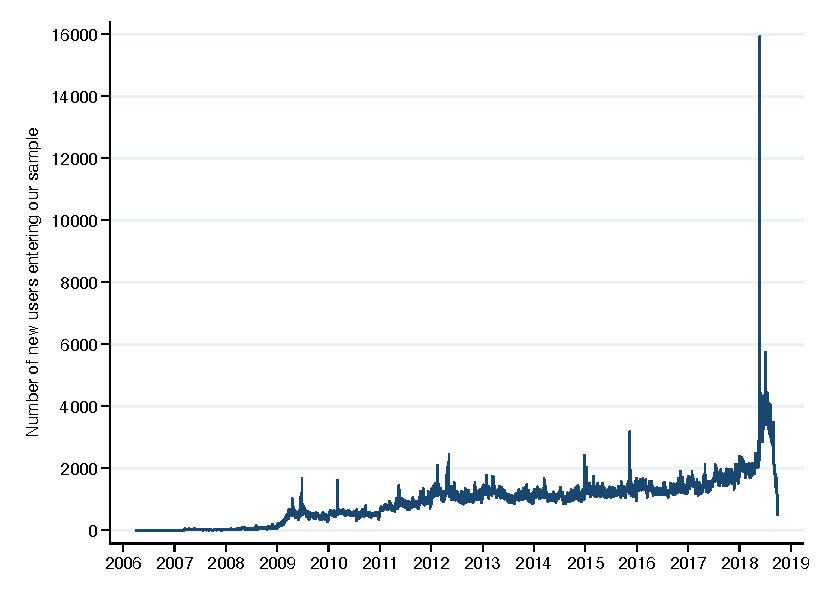
\includegraphics[scale=1]{figures/fig_nb_new_users_daily}
\end{center}
	\begin{spacing}{0.5}
		{\footnotesize \textbf{Notes:} The figure plots the number of users entering our sample depending on the date of their Twitter account creation.}
	\end{spacing}
\vspace{.5cm}	
	\caption{Twitter users: Number of followers depending on the date of their account creation}
	\label{fig:fig_nb_new_users_daily}
\end{figure}
%%%%%%%%%%%%%%%%%%%%%%%%%%%%%%%%%%%%%%%%%%%%%%%%%%%%%%%%%%%%%%%%%%%%%% 


%%%%%%%%%%%%%%%%%%%%%%%%%%%%%%%%%%%%%%%%%%%%%%%%%%%%%%%%%%%%%%%%%%%%%%
\clearpage
\pagebreak
\begin{figure}
\begin{center}
	\subfloat[][\textbf{Distribution of the number of followers}]{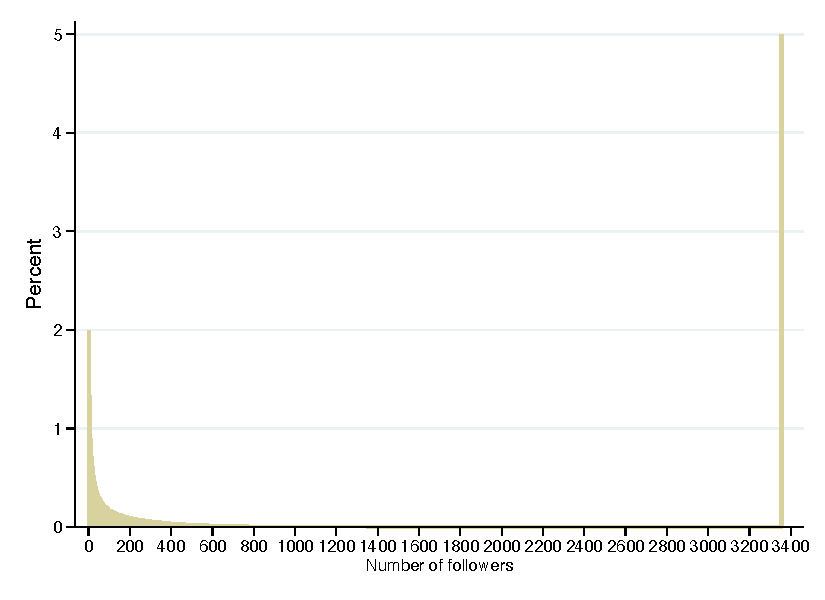
\includegraphics[scale=.9]{figures/distribution_users}
\label{fig:distribution_users}}
\quad
	\subfloat[][\textbf{Cumulative distribution of the number of followers}]{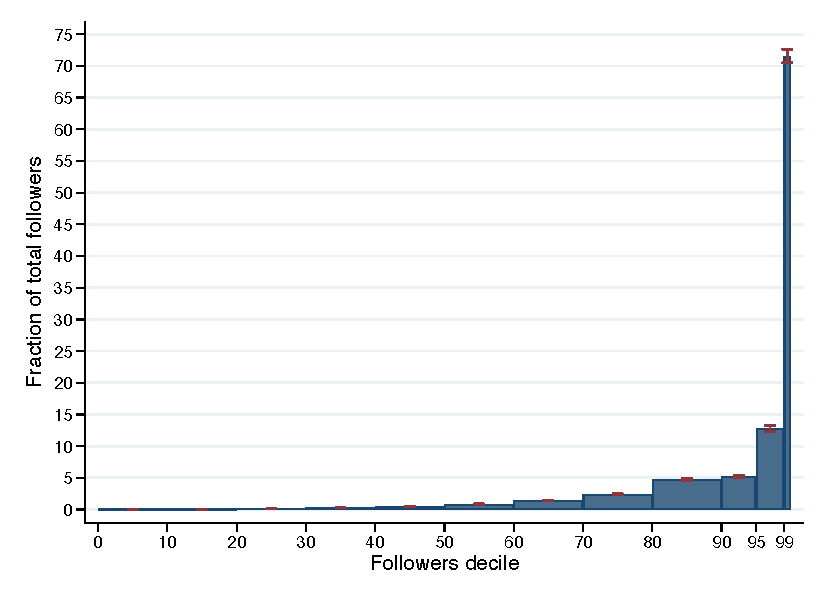
\includegraphics[scale=.9]{figures/cumulative_distribution_followers}
\label{fig:cumulative_distribution_followers}}
\end{center}
	\begin{spacing}{0.5}
		{\footnotesize \textbf{Notes:} The upper Figure \ref{fig:distribution_users} plots the distribution of the number of followers (winsorized at the 95th percentile, i.e. $3,355$ followers) of the Twitter users in our dataset. The bottom Figure \ref{fig:cumulative_distribution_followers} plots the cumulative distribution of the number of followers.}
	\end{spacing}
\vspace{.5cm}	
	\caption{Twitter users: Distribution of the number of followers}
	\label{fig:users}
\end{figure}
%%%%%%%%%%%%%%%%%%%%%%%%%%%%%%%%%%%%%%%%%%%%%%%%%%%%%%%%%%%%%%%%%%%%%% 


%%%%%%%%%%%%%%%%%%%%%%%%%%%%%%%%%%%%%%%%%%%%%%%%%%%%%%%%%%%%%%%%%%%%%%
\clearpage
\pagebreak
\begin{figure}
\begin{center}
	\subfloat[][All documents]{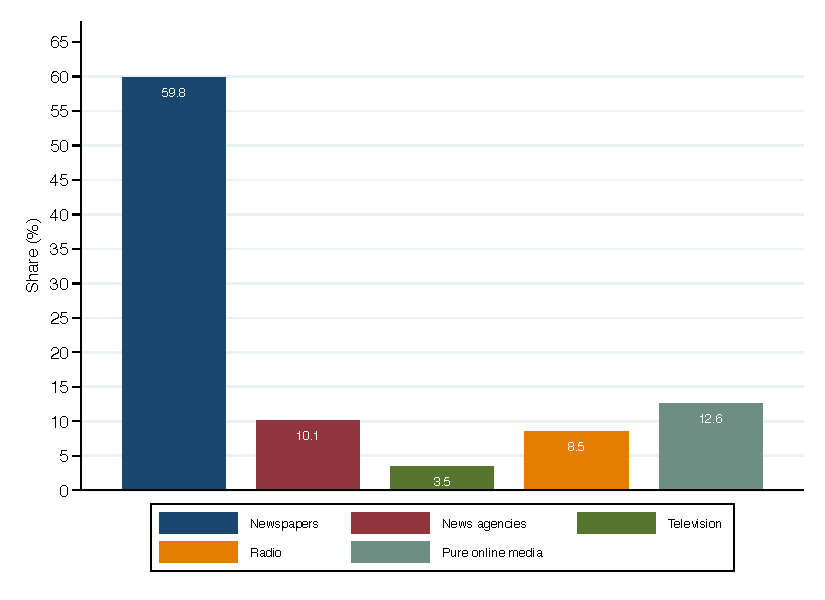
\includegraphics[scale=.6]{figures/share_documents_used_media_category_m}
\label{fig:share_documents_used_media_category_m}}
\quad
	\subfloat[][Documents classified in events]{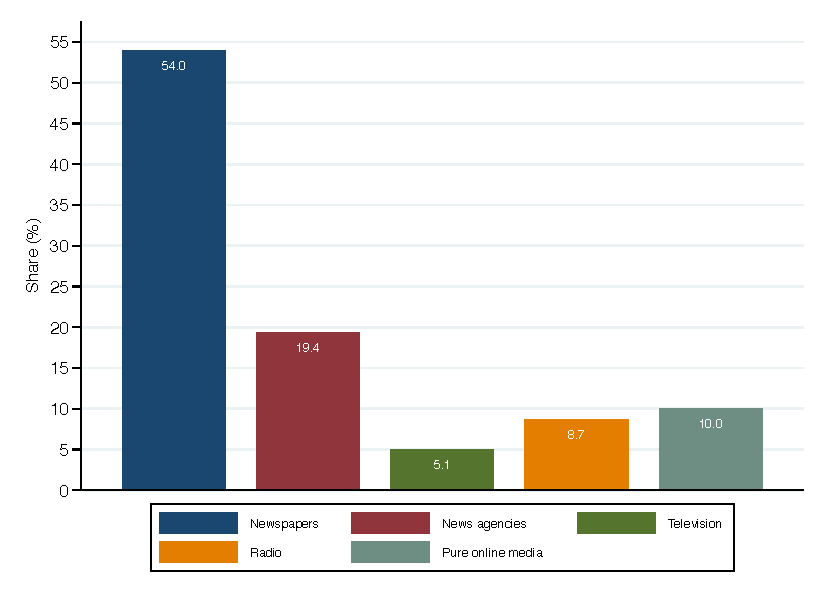
\includegraphics[scale=.6]{figures/share_documents_used_media_category_m_C}
\label{fig:share_documents_used_media_category_m_C}}
\quad
	\subfloat[][Documents not classified in events]{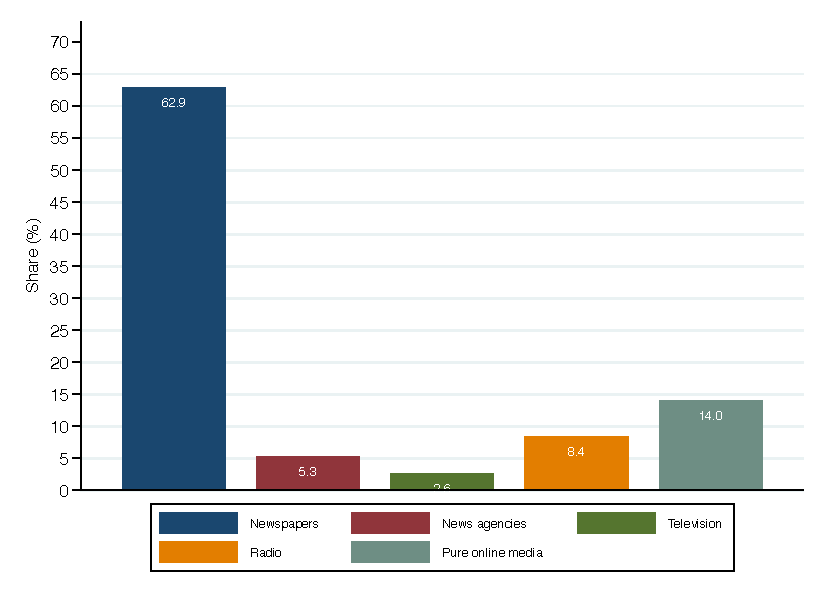
\includegraphics[scale=.6]{figures/share_documents_used_media_category_m_NC}
\label{fig:share_documents_used_media_category_m_NC}}
\end{center}
	\begin{spacing}{0.5}
		{\footnotesize \textbf{Notes:} The figures plot the share of the documents depending on the offline format of the media outlet. The upper figure \ref{fig:share_documents_used_media_category_m} plots this number for all the documents; the middle figure \ref{fig:share_documents_used_media_category_m_C} for the documents classified in events; and the bottom figure \ref{fig:share_documents_used_media_category_m_NC} for the documents not classified in events. News events are defined in detail in the text, and the list of the media outlets included in each category is given in Section \ref{Sec:Sources}.}
	\end{spacing}
\vspace{.5cm}	
	\caption{Share of the documents by offline format}
	\label{fig:share_documents_used_media_category}
\end{figure}



%%%%%%%%%%%%%%%%%%%%%%%%%%%%%%%%%%%%%%%%%%%%%%%%%%%%%%%%%%%%%%%
\begin{figure}
\begin{center}
\subfloat[][\textbf{English}]{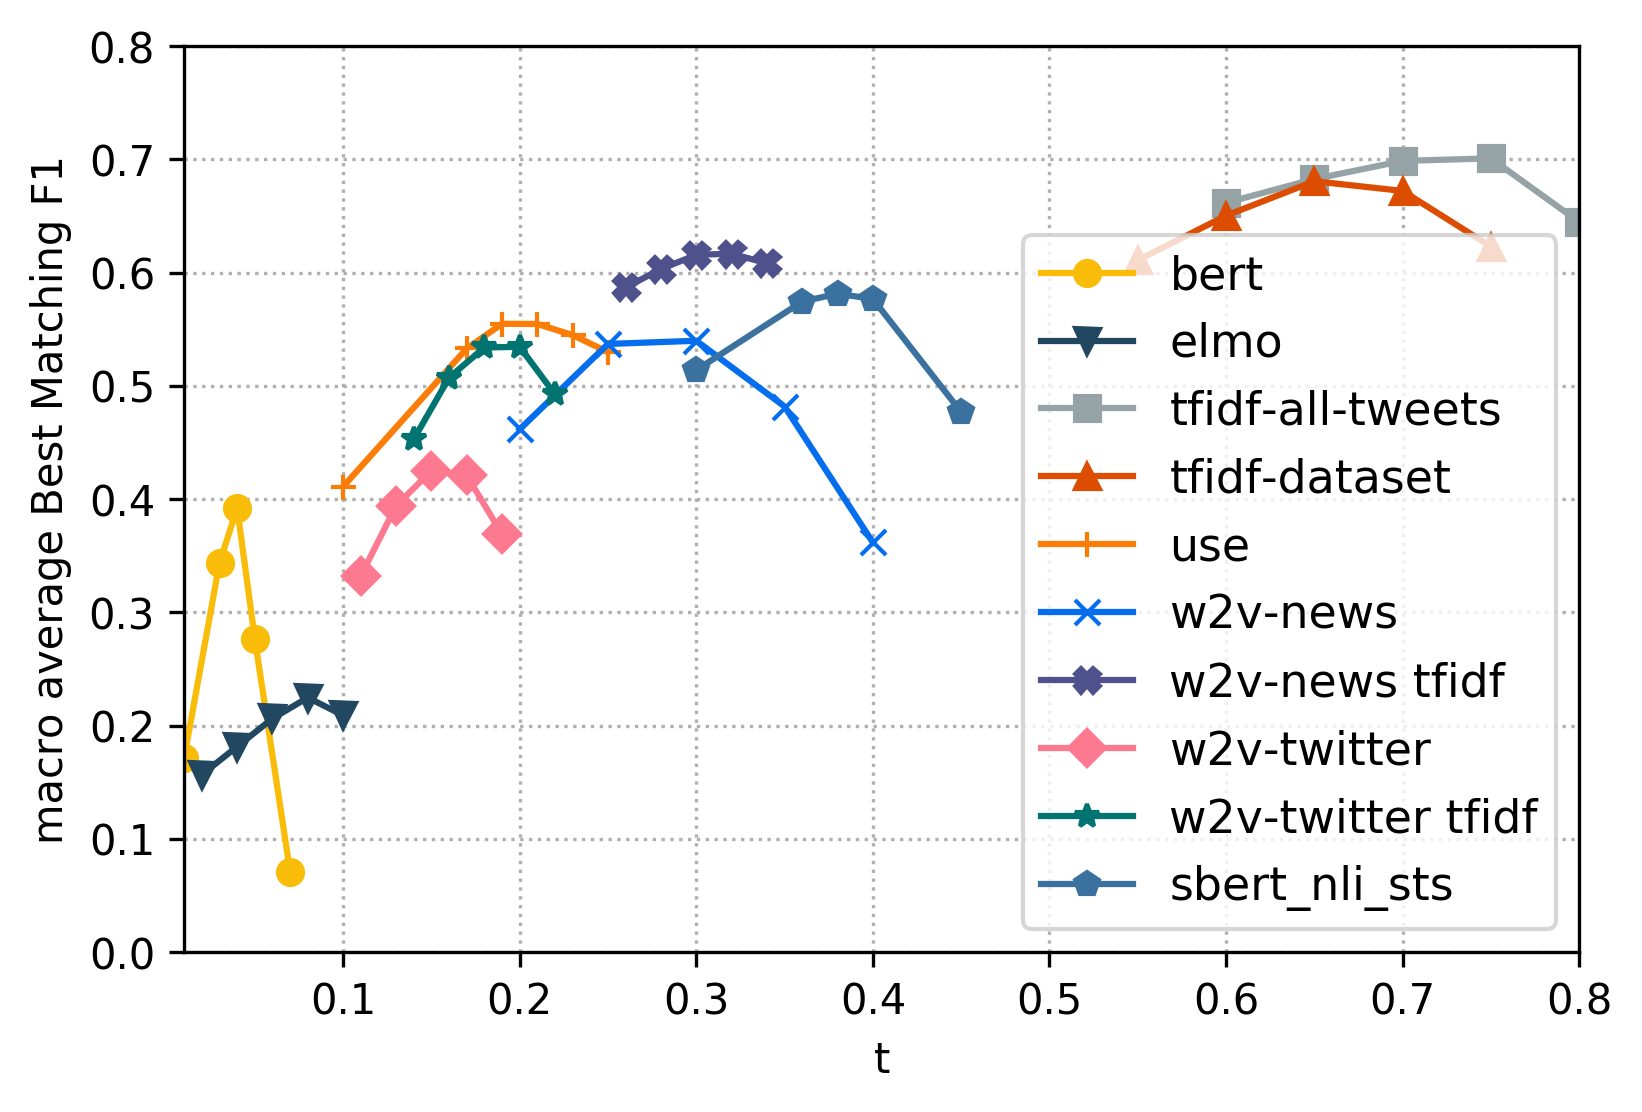
\includegraphics[width=1\linewidth]{figures/Beatrice/graph_en_FSD.png}
\label{fig: graph_FSD_en}}
\quad
\subfloat[][\textbf{French}]{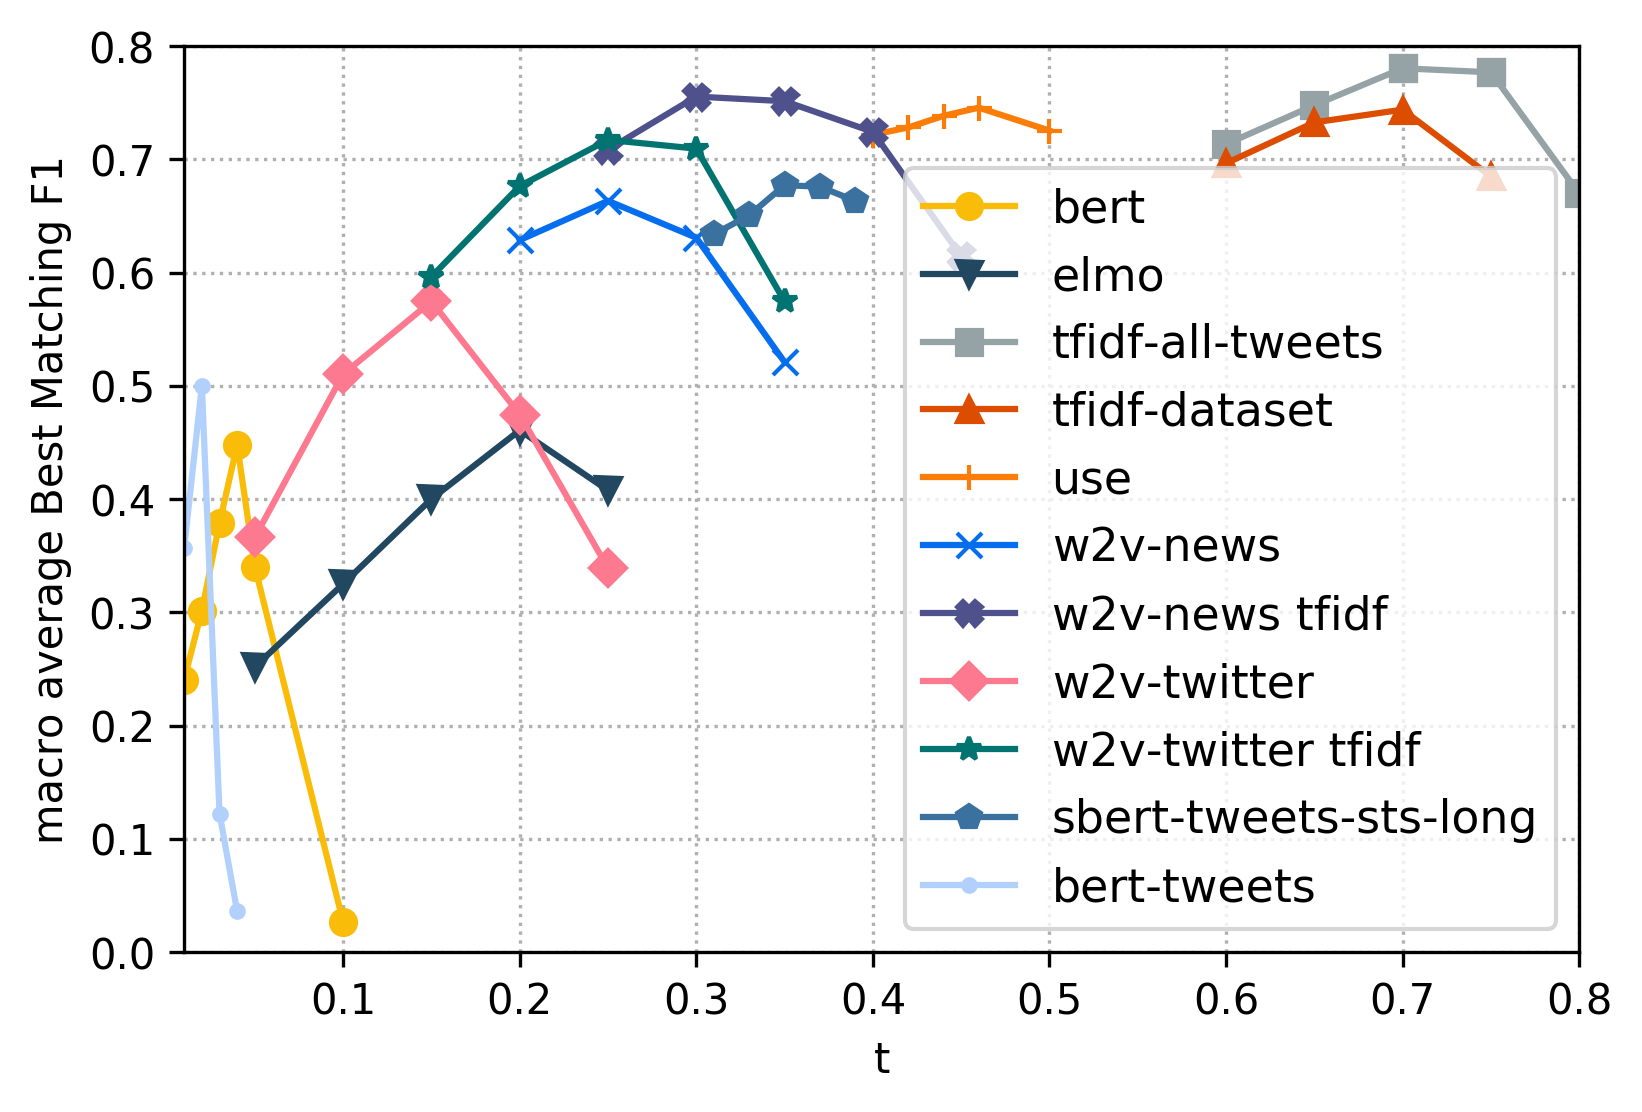
\includegraphics[width=1\linewidth]{figures/Beatrice/graph_fr_FSD.png}
\label{fig: graph_FSD_fr}}
\end{center}
\caption{Best Matching F1 score for FSD clustering depending on the threshold parameter $t$ for each corpus}
\label{fig: graph_FSD}
\end{figure}
%%%%%%%%%%%%%%%%%%%%%%%%%%%%%%%%%%%%%%%%%%%%%%%%%%%%%%%%%%%%%%


%%%%%%%%%%%%%%%%%%%%%%%%%%%%%%%%%%%%%%%%%%%%%%%%%%%%%%%%%%%%%%%%%%%%%%
\clearpage
\pagebreak
\begin{figure}
\begin{center}
	\subfloat[][Fourth quartile of the number of articles distribution]{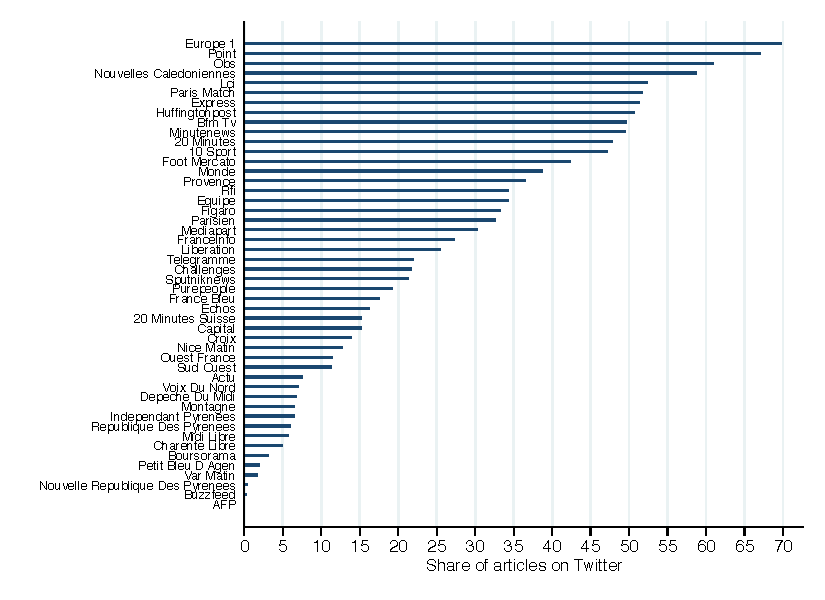
\includegraphics[scale=.6]{figures/fig_mean_Tweeted_fourth_quartile_nb_articles}
\label{fig:fig_mean_Tweeted_fourth_quartile_nb_articles}}
\quad
	\subfloat[][Third quartile of the number of articles distribution]{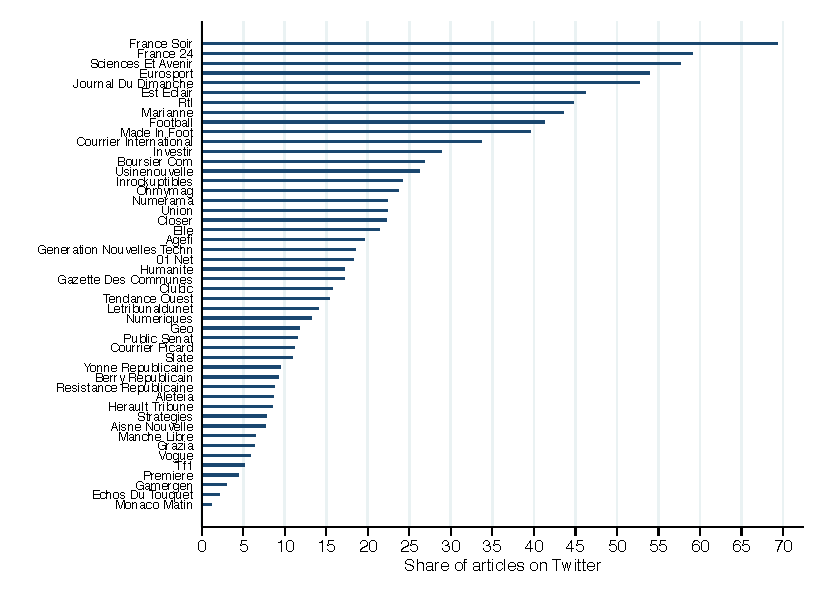
\includegraphics[scale=.6]{figures/fig_mean_Tweeted_third_quartile_nb_articles}
\label{fig:fig_mean_Tweeted_third_quartile_nb_articles}}
\quad
	\subfloat[][Second quartile of the number of articles distribution]{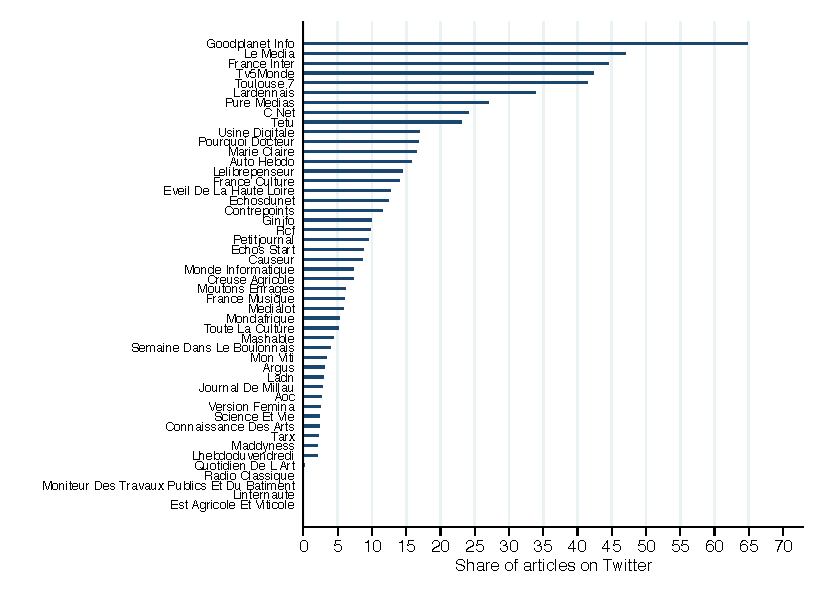
\includegraphics[scale=.6]{figures/fig_mean_Tweeted_second_quartile_nb_articles}
\label{fig:fig_mean_Tweeted_second_quartile_nb_articles}}
\end{center}
	\begin{spacing}{0.5}
		{\footnotesize \textbf{Notes:} The figures plot the share of the articles published online that are on Twitter, depending on the media outlet. Media outlets are ranked depending on the number of articles they publish online between July 2018 and September 2018. The upper figure \ref{fig:fig_mean_Tweeted_fourth_quartile_nb_articles} plots the share for the media outlets that are in the fourth quartile of the number of articles distribution; the middle figure \ref{fig:fig_mean_Tweeted_third_quartile_nb_articles} for the media outlets that are in the third quartile; and the bottom figure \ref{fig:fig_mean_Tweeted_second_quartile_nb_articles} for the media outlets that are in the second quartile.}
	\end{spacing}
\vspace{.5cm}	
	\caption{Share of the articles published online that are on Twitter, depending on the media outlet}
	\label{fig:fig_mean_Tweeted}
\end{figure}


%%%%%%%%%%%%%%%%%%%%%%%%%%%%%%%%%%%%%%%%%%%%%%%%%%%%%%%%%%%%%%%%%%%%%%
\clearpage
\pagebreak
\begin{figure}
\begin{center}
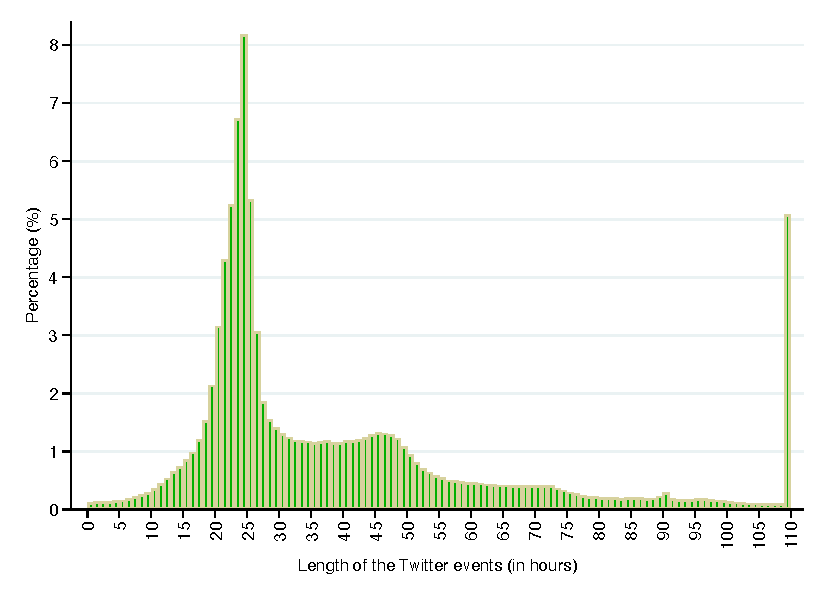
\includegraphics[scale=1]{figures/distribution_length_Tevents}
\end{center}
	\begin{spacing}{0.5}
		{\footnotesize \textbf{Notes:} The figure plots the distribution of the length of the Twitter events (in hours), Winsorized at the 95th percentile (=105 hours). \textbf{REPRENDRE PROPEMENT}}
	\end{spacing}
\vspace{.5cm}	
	\caption{ Twitter events: Distribution of the length of the events (in hours),
Winsorized at the 95th percentile (=109.8 hours)}
	\label{fig:distribution_length_Tevents}
\end{figure}
%%%%%%%%%%%%%%%%%%%%%%%%%%%%%%%%%%%%%%%%%%%%%%%%%%%%%%%%%%%%%%%%%%%%%% 



% %%%%%%%%%%%%%%%%%%%%%%%%%%%%%%%%%%%%%%%%%
% %%%%%%%%%%%%%%%%%%%%%%%%%%%%%%%%%%%%%%%%% 
% \clearpage
% \pagebreak 
% \bibliographystyle{aer}
% \bibliography{../twitter_bib}
% \pagebreak

% \end{document}
